\documentclass{book}


\usepackage{elsst-book}
\usepackage{float}
\usepackage{amsmath}
\usepackage{amsfonts}
\usepackage{graphicx}
\usepackage{lineno}
\usepackage{natbib}
\usepackage{hyperref}
\usepackage{verbatim}
\usepackage{soul}
\usepackage{color}
\usepackage{bm}

\bibliographystyle{asa}


\floatstyle{plain}
\floatname{panel}{Panel}
\newfloat{algorithm}{h}{txt}[chapter]
\newfloat{panel}{h}{txt}[chapter]

\linenumbers

\begin{document}



%\chapter{Introduction}
%\label{chapt.intro}

%\chapter{
Introduction to Spatial Capture-Recapture
}
\markboth{Introduction}{}
\label{chapt.intro}

\vspace{.3in}



Space: The final frontier. The spatial structure of populations, and
spatial processes that contribute to population dynamics,  
are central to  applied and theoretical population ecology.  At the
same time, the inherent spatial aspect of {\it sampling} populations
strongly affects apprent biases in how we observe population structure.
Books have been written on spatial processes in animals
oppulations \citep{tilman_kareiva:1997,hanski:1999}
and books have been written on how we sample these populations using
capture-recapture methods \citep{seber:1982,williams_etal:2003}.

Despite the central roll of space and spatial processes to both
understanding population dynamics and to how we observe population
structure, these two things have not yet been synthesized....... We do that
here, in this book.


Spatial processes structure animal populations --
-- movement, spatial variation in density, space usage, density dependence, interactions among individuals.
This is all about motive -- should not be about fixing technical
problems
with existing estimators but , rather, modeling actual ecological
processes.

SCR is about explicit formulations of CR models that involve space --
the spatial context of how we observe individuals , and what gives
rise to the distribution of individuals in space, and how individuals
use space, etc... 





\section{Capture-Recapture}

Information about abundance or density of populations, and their vital
rates, is fundamental to applied ecology and conservation biology.  To
that end, a huge variety of statistical methods have been devised, and
among these, the most well-developed are collectively known as
capture-recapture (or capture-mark-recapture) methods. For example,
the volumes by \citet{seber:1982}, \citet{borchers_etal:2002},
\citet{williams_etal:2002}, and \citet{amstrup_etal:2005} are largely
synthetic treatments of such methods, and contributions on modeling
and estimation using capture-recapture are plentiful in the
peer-reviewed ecology literature.  

Capture-recapture techniques have been the number 1 quantiative method
in studies of animal populations for decades.
But they apply basically to fish bowl sampling. Does it make sense
that methods should apply to both?

Capture-recapture techniques make
use of individual encounter history data, by which we mean sequences
of 0's and 1's denoting if an individual was encountered at a
particular trap during a certain time period. For example, the
encounter history ``010'' indicates that this individual was
encountered only during the second of three trapping occasions. As we
will see, these data contain
information about encounter probability, abundance, and other
parameters of interest in the study of population dynamics.

A diverse and growing number of methods exist for obtaining encounter
history data. Such methods are, naturally, taxa-specific. They include
classical ``traps'' which capture and retain animals until visited by
a biologist who removes the individual, marks it, or otherwise molests
it in some scientific fashion.  Small-mammal traps and mist nets for
birds are standard examples. Traps that physically capture and
restrain individuals are common, but capture-recapture methods no
longer require ``capture'' or even physical marking of individuals.
Recent technological advances have produced a
large number of passive detection devices that produce individual
encounter history data. These include camera traps
\citep{karanth_nichols:1998, oconnell_etal:2010}, acoustic recording
devices \citep{dawson_efford:2009}, and methods that obtain DNA
samples such as hair snares for bears \citep{gardner_etal:2010jwm}, scent
posts for many carnivores \citep{kery_etal:2010}, and related methods which allow DNA
to be extracted from scat, urine or animal tissue in order to identify
individuals.  This book is concerned with how such data can be used to
carry out inference about animal abundance or density, and other
demographic parameters such as survival, recruitment, and movement
using new classes of capture-recapture models which utilize auxiliary
spatial information related to the encounter process.  We refer to
such methods as spatial capture-recapture (SCR) models\footnote{In
the literature the term spatially explicit capture-recapture (SECR) is
also used}.

As the name implies, the primary feature of SCR models that
distinguishes them from traditional CR methods is that they make use
of the spatial information inherent to capture-recapture studies. That
is, the encounter histories are associated with spatial coordinates,
and these coordinates are informative about home range
characteristics, movement and space usage.
As we will see, this allows us to overcome three critical
deficiencies of non-spatial methods, namely,
traditional CR methods cannot be used to formally estimate density,
include of trap-level covariates of density or capture probability, or
account for heterogeneity in encounter probability that
results from the spatial organization of animals and traps.
Thus, spatial modeling is not just
a fun academic exercise; it provides a solution to basic problems in
the study of animal populations that have been acknowledged for more
than 70 years \citep{dice:1938}.
More important than just providing a resolution to
some basic technical problems,
SCR models provide
 a framework
for integrating
into capture-recapture models
explicit ecological hypotheses related to space usage,
and the spatial
organization of individuals in a population.
This greatly expands the practical utility and scientific
relevance of
capture-recapture methods and studies based on
encounter history data.

\section{Scope of this Book}

In this book, we try to achieve a broad methodological scope from
basic closed population models %using a number of distinct observation
%models
for inference about population density on up to open population models
for inference about vital rates such as survival and recruitment. %---spatial versions of
%conventional Jolly-Seber models. %A number of conceptual and
%methodological themes unify the main topical coverage of this book, and
%those are:
Much of the material is a synthesis of recent research but we also expand SCR models in a
number of useful directions, including to accomodate unmarked individuals
(Chapt. \ref{chapt.xxxx}), use of telemetry information (Chapt. \ref{chapt.rsf}), and developing
explicit models of individual space usage (Chapt. \ref{chapt.ecoldist}), and many other
new topics that have yet to appear in the literature.
Our intent is to
provide a comprehensive resource for ecologists interested in
understanding and applying SCR models to solve common problems
faced in the study of population dynamics. To do so, we make use of
hierarchical models, which allow extraordinary
flexibility in accommodating virtually any type of capture-recapture
data. We present many example analyses, of real and simulated data
using likelihood-based and Bayesian methods---examples that readers
can replicate using the code presented in the text and
the resources made available on-line and in our accompanying {\bf R} package
{\tt scrbook}.

Although we aim to reach a
broad audience, at times we go into details that may only be of
interest to advanced practitioners who need to extend these models to
unique situations.  We hope that these advanced topics will not
discourage those new to these methods, but instead we believe this
material will allow readers to advance their understanding and become
less reliant on restrictive tools and software. Before discussing the
specifics of SCR models, we begin with an overview of the methods
used to collect capture-recapture data, and provide a brief summary of
traditional non-spatial capture-recapture models.



In this book we present a diverse array of modeling approaches for making
inference about density and population dynamics using spatial
capture-recapture data. A number of conceptual and
methodological themes unify the main topical coverage of this book, and
those are:

\begin{itemize}
\item[(1)] Hierarchical modeling. We develop hierarchical models
  consisting of explicit models for both the observation process and
  the underlying ``ecological process'' which describes the
  organization of individuals in space.

\item[(2)] Formal inference using both classical (frequentist,
  likelihood-based) and Bayesian methods. We often emphasize
  Bayesian analysis because this allows us to focus the technical
  formulation of models, and spatial capture-recapture is mainly
  concerned with modeling random effects and estimating functions of
  random effects. However, we also explore likelihood methods using existing
  software such as the R package SECR \citep{efford:2011}, as well as
  development of custom solutions along the way.

\item[(3)] In developing Bayesian analyses of SCR models, we emphasize
  the use of the BUGS language for describing models. The BUGS
  language emphasizes the syntactic description of the essential
  assumptions of models in a special kind of pseudo-code language,
  which is used in software (WinBUGS, JAGS, OpenBUGS) to devise Markov
  chain Monte Carlo (MCMC) algorithms for Bayesian analysis of
  models. The BUGS language focuses your thinking on model development
  and lets you develop an understanding of models at the level of
  their basic assumptions and structure.  Despite our focus on
  describing models using the BUGS language, we also show readers how
  to devise their own MCMC algorithms for Bayesian analysis of SCR
  models, which can be convenient (even necessary) in some practical
  situations.

\item[(4)] Data augmentation -- dealing with the fact that population
  size, $N$, is unknown is a challenging technical problem in
  capture-recapture models. We confront this problem in almost every
  chapter of this book. To deal with it we use a technical device
  called {\it data augmentation} which is extremely useful for
  analysis of capture-recapture models that are specified
  ``conditional on $N$'' \citep{royle_etal:2007}.
\end{itemize}

Altogether, these different conceptual and methodological elements
provide for a formulation of SCR models that essentially renders them
as variations of generalized linear mixed models (GLMMs). This in a
sense makes them consistent with many important methodologies used in
ecology (e.g., see \citet{zuur_etal:2009, kery_etal:2010}), and
because of the connection with standard modeling concepts, we believe
that the material presented in this book can be understood and used by
most ecologists with some modeling experience.

This book is not a book about Bayesian analysis, not a book about
hierarchical models, not a book about capture-recapture, and not about
programming in R. In a sense though, our book integrates elements of
all of these things into what we hope is a coherent package for
analyzing data from this enormous class of data collection methods
that produce spatially-explicit capture-recapture data.   As such, we
expect that people have a basic understanding of statistical models
and classical inference (What is frequentist inference? what is a
likelihood? Generalized linear model? Generalized linear mixed
model?),
{\bf R} programming,
 Bayesian analysis (what is s a prior distribution and a
posterior distribution?),
and maybe even a little bit
of Bayesian
computation (MCMC and perhaps the BUGS language).
The ideal candidate for reading this book has basic knowledge of these
topics. However, we do provide introductory chapters on the necessary
components which we hope can serve as a brief and cursory tutorial for
those who might have only limited technical knowledge, e.g., many
carnivore biologists who implement field sampling programs but do not
have extensive experience analyzing data.



\section{Lions and Tigers and Bears, oh my:  Genesis of
Spatial capture-recapture data}

A diverse number of methods and devices exist for producing individual
encounter history data with auxiliary spatial information about
individual locations. Historically, physical ``traps'' have been widely
used to sample animal populations. These include live traps, leg-hold
traps, mist nets, pitfall traps and many other types of
devices. Although these are still widely used, 
recent technological advances 
for obtaining encounter history
data non-invasively 
 have made it possible to study many species that
were difficult if not impossible to study effectively just a few years
ago.  And, 
 we believe, these methods have revolutionized the study of animal populations by
 capture-recapture methods and will lead to their increasing
 relevance in the future.
 We briefly review some of these here, which we
 consider more explicitly in later chapters of this book.

\subsection{Camera trapping}

Considerable recent work has gone into the development of
camera-trapping methodologies. For a historical overview of this
method see \citet{kays_etal:2008} and \citet{kucera_barrett:2011}.  Several
recent synthetic works have been published including
\citet{nichols_karanth:2002}, and an edited volume by
\citet{oconnell_etal:2010} devoted solely to camera trapping concepts
and methods. As a method for estimating abundance, some of the earliest
work that relates to the use of camera trapping data in
capture-recapture models originates from Karanth and colleagues
\citep{karanth:1995, karanth_nichols:1998, karanth_nichols:2000}. In
camera trapping studies, cameras are situated along trails or
at baited stations and individual animals are photographed and
subsequently identified either manually by a person sitting behind a
computer,  or sometimes now using computational
methods. Camera trapping methods are widely used for species that have
unique stripe or spotting patterns such as tigers \citep{karanth:1995,
  karanth_nichols:1998}, ocelots
\citep{trolle_kery:2003,trolle_kery:2005}, leopards
\citep{balme_etal:2010}, and many other cat species.
% Scientific names
Camera traps are
also used for other species such as wolverines 
\citep[{\it Gulo gulo}][]{magoun_etal:2011,royle_etal:2011}, 
and even species that are less easy to
identify uniquely such as mountain lions \citep{sollmann_etal:inprep} 
and coyotes  %add scientific names
(e.g. \citet{kelly_etal:2008}.  We note that even for species that are
not readily identified by pelage patterns, it might be efficient to use
camera traps in conjunction with spatial capture-recapture models to
estimate density (see Chapt.~\ref{chapt.scr-unmarked}).
%, if an initial sample of individuals can be collared
%or tagged in some way so that subsequent encounter by camera-traps can
%yield individual information. In this way, the probability of
%encounter can be estimated from the camera traps based on the
%pre-marked individuals, and this is applied to the frequencies of
%unmarked individuals to estimate density.


\begin{figure}
\begin{center}
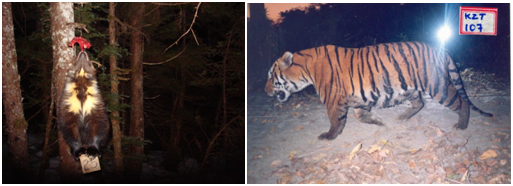
\includegraphics[width=5in]{Ch1/figs/wolverinetiger}
\end{center}
\caption{
Left: Wolverine being encounter by a
camera trap ({\it Photo credit: Audrey Magoun}).
Right: Tiger encountered by
camera trap ({\it Photo credit: Ullas Karanth/WCS}).
}
\label{fig.wolverinetiger}
\end{figure}

\subsection{DNA Sampling}

DNA obtained from hair, blood or scat is now
routinely used to obtain individual identity and encounter history
information about individuals \citep{taberlet_bouvent:1992,
  woods_etal:1999, mills_etal:2000, schwartz_monfort:2008}.  A common
method is based on the use of ``hair snares'' (Fig. \ref{fig.bearcat})
which are widely used to study bear populations
\citep{woods_etal:1999, gardner_etal:2010jwm, garshelis_etal:2006,
  kendall_etal:2009}.  A sample of hair is obtained as individuals
pass under or around barbed-wire (or other physical mechanism) to take
bait. Hair snares and scent sticks have also been used to sample felid populations
\citep{garciaalaniz_etal:2010, kery_etal:2010} and other species. Research has even shown that
DNA information can be extracted from urine deposited in the wild (e.g., in snow; see \cite{valiere_taberlet:2000})
and as a result this may prove another future data collection technique where SCR models
are useful.

\begin{figure}
\begin{center}
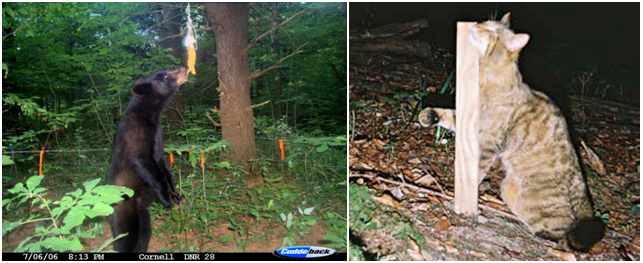
\includegraphics[width=5in]{Ch1/figs/bearcat}
\end{center}
\caption{Left:  Black bear in a hair snare ({\it Photo credit: M. Wegan})
Right: European wildcat loving on a scent stick ({\it Photo credit: Darius
Weber, Hintermann \& Weber AG, Ecological Consultancy, Planning \&
Research, Switzerland})
}
\label{fig.bearcat}
\end{figure}


\begin{figure}
\begin{center}
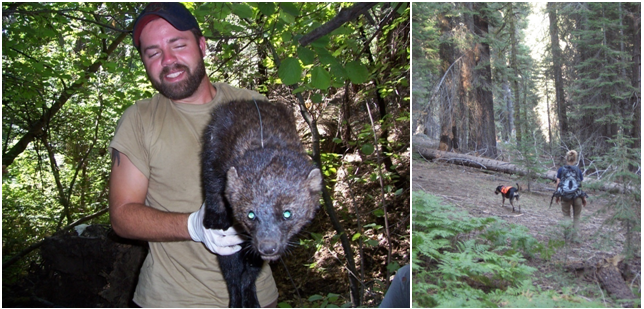
\includegraphics[width=5in]{Ch1/figs/beardog}
\end{center}
\caption{Left:
A wildlife research technician for the USDA Forest Service
  holding a male fisher  captured as part of the Kings River Fisher
  Project in the Sierra National Forest, California.
Right: A dog handler surveying for fisher scat in the Sierra National Forest.
{\it Photo credit: Craig Thompson, USDA Forest Service,
Pacific Southwest Research Station.}}
\label{fig.fisherscatdog}
\end{figure}


\subsection{Acoustic surveys}

Many studies of birds \citep{dawson_efford:2009}, bats, and whales \citep{marques_etal:2009}  now collect data using
devices that record vocalizations. When vocalizations can be identified by individual from multiple
recording devices, spatial encounter histories are produced that are amenable to
the application of SCR models \citep{dawson_efford:2009, efford_etal:2009ecol}.

\subsection{Search-Encounter Methods}

There are other methods which don't fall into a nice clean taxonomy of
``devices''. Spatial encounter histories\footnote{defined? probably
  not! need to do that} are commonly obtained by conducting manual
searches of geographic sample units such as quadrats, transects or
road or trail networks.
For example,
DNA-based encounter histories can be obtained from scat
samples located along roads or trails or by specially trained dogs
\citep{mackay_etal:2008} searching space
(Fig. \ref{fig.fisherscatdog}). This method has been used in studies
of martens, fishers \citep{thompson_etal:inpress}, lynx, coyotes,
birds \citet{kery_etal:2010}, and many other species. We might search
space on foot and pick up individuals and physically mark them
somehow. This is pretty common in surveys that involve reptiles and
amphibians, e.g., we might walk transects picking up 
box turtles \citep{hall_etal:1999}, or desert tortoises \citep{zylstra_eta:2010},
 or search space for lizards
\citep{royle_young:2008} and also surveys designed to obtain animal
scat. These methods don't seem like normal capture-recapture in the
sense that the encounter of individuals is not associated with
specific trap location, but SCR models are equally relevant for
analysis of such data (see Chapt. \ref{chapt.searchencounter}).


\section{ Historical Context: A Brief Synopsis of the Literature}

Spatial capture-recapture is a relatively new methodological
development, at least with regard to formal estimation and
inference. However, the basic problems that motivate the need for
formal spatially-explicit models have been recognized for decades and
quite a large number of ideas have been proposed to deal with these
problems. We review some of these ideas here.


\subsection{Buffering}

 The standard approach to estimating density even now is to estimate $N$ using
conventional closed population models \citep{otis_etal:1978} and then
try to associate with this estimate some specific sampled area, say $A$,
the area which is contributing individuals to the population for which
$N$ is being estimated. The strategy is to define $A$ by placing a buffer
of say $W$ around the trap array or some polygon which encloses the trap
array. The historical context is succinctly stated by \citep{obrien:2011}
from which we draw this description:

\begin{quote}
  ``At its most simplistic, $A$ may be described by a concave polygon
  defined by connecting the outermost trap locations ($A_{tp}$; \citet{mohr:1947}).
 This assumes that animals do not move from outside the
  bounded area to inside the area or vice versa. Unless the study is
  conducted on a small island or a physical barrier is erected in the
  study area to limit movement of animals, this assumption is unlikely
  to be true. More often, a boundary area of width $W$ ($A_{w}$) is added to
  the area defined by the polygon $A_{tp}$ to reflect the area beyond the
  limit of the traps that potentially is contributing animals to the
  abundance estimate \citep{otis_etal:1978}. The sampled area, also known
  as the effective area, is then $A(W) = A_{tp} + A_{w}$. Calculation of the
  buffer strip width ($W$) is critical to the estimation of density and
  is problematic because there is no agreed upon method of estimating
  $W$. Solutions to this problem all involve ad hoc methods that date
  back to early attempts to estimate abundance and home ranges based
  on trapping grids
  \citep[see][]{hayne:1949}. \citet{dice:1938} first drew attention
  to this problem in small mammal studies and recommended using
  one-half the diameter of an average home range. Other solutions have
  included use of inter-trap distances \citep{blair:1940,burt:1943}, mean
  movements among traps, maximum movements among traps \citep{holdenried:1940, hayne:1949},
 nested grids \citep{otis_etal:1978}, and assessment
  lines \citep{smith_etal:1971}.''
\end{quote}

The idea of using 1/2 mean maximum distance moved
\citep{wilson_anderson:1985a} seems to be the standard approach even
today, presumably justified by Dice's suggestion to use 1/2 the home
range diameter. Alternatively, some studies have used the full
MMDM (e.g. \citet{parmenter_etal:2003}),

%\footnote{Do they really say that?}  Yes, they really do use it, but so
%do a lot of studies so we can add more if you want.

because the trap array might not provide a full coverage of the home range so 1/2 MMDM may be smaller than the home range radius. And, sometimes home range size is
estimated by telemetry \citep{karanth:1995, bales_etal:2005}.
%\footnote{Is this correct cite for this?}.  Karanth used some technique, it's hard to tell for sure....but he
% mentions using 1 female that is collared to estimate effective trap area.  Bales does it too, so I added it for
% extra value!

This is usually combined
with an AIC-based selection from among the closed-population models in
\citet{otis_etal:1978} which most often suggests heterogeneity in detection (Model
Mh).  Almost all of these early methods were motivated by studies of
small mammals using classical ``trapping grids'' but, more recently,
their popularity has increased with the advent of new technologies and
especially related to non-invasive sampling methods such as camera
trapping. In particular, the series of papers by Karanth and Nichols
\citep{karanth:1995, karanth_nichols:1998, karanth_nichols:2002}
has led to fairly widespread adoption of these ideas.

Some of the heuristic ideas based on buffer strips do have some
technical justification in the sense of estimating parameters of an
underlying movement model from observed movements. For example, if we
let $x$ be a random variable indicating movement outcomes of an
individual about its  home range center, and suppose that $x$ has pdf
$g(x)$ then we can understand properties of MMDM by studying the
properties of the sample order statistics, as the maximum distance
moved is the sample range based on a sample of observations of
individual locations.



%As an illustration, imagine a 1-dimensional
%system where individuals have a home range that amounts to a line
%segment. Then suppose that individual movements are $\mbox{uniform}(0,A)$. It
%can be shown that the sampling distribution of the sample range, R,
%scaled by $A$, say $R/A$ has a beta distribution, $\mbox{beta}(n-1,2)$
%\citep[][p. 235]{casella_berger:2002}
%and thus the diameter of the home range, i.e. $A$, is
%estimated (biasedly) by$ R/( (n-1)/(n+1) )$. For large $n$ we could then
%say that the sample range, i.e., ''maximum distance moved'' seems like a good estimator of home range diameter and, therefore, $R/2$ is an estimator of home-range radius.

%There are a number of technical issues that arise in attempting to use
%such heuristics to justify the application in practice. For one, the
%moments of the sample order statistics are strongly affected by sample
%size, which is typically quite small (per individual encountered) and
%thus, in general, are biased and estimated with variable precision
%depending on sample size. For example, the expected value of MMDM is
%$k(n)*A$ , i.e., the true home range diameter is related to observed
%MMDM by some function of sample size, $k(n)$, that increases to 1. In
%the case where the underlying movement model is uniform, $k(n) =
%(n-1)/(n+1)$ (from above) which motivates a formula for ``adjusting''
%observed MMDM for small sample size. We suspect that many such
%formulae are obtainable depending on the assumed movement distribution
%\citep[e.g., formula 6.16 in][]{obrien:2011}. We might also think about taking
%the {\it maximum} (over individuals) of the maximum distance moved
%because under the specific model considered here (iid uniform) then
%all individuals have the same home range radius. This increases our
%sample size ($n$) and thus the observed sample range should be more
%accurate.


%%Another issue of somewhat more importance (and less easy to
%rectify) is that the {\it observation} of movement outcomes is biased
%by the locations of traps. We cannot observe movements ``off the
%trapping grid'' (or between traps) and thus our observed movements
%will generally be smaller than expected under any particular model
%(the uniform in this case). Moreover, the trap spacing also induces a
%discreteness to the movements that causes a further level of
%approximation based on hypothetical movement
%distributions. Nevertheless, formal analysis of `` buffering''
%strategies based on sample order statistics under specific models for
%movement does at least provide some heuristic support for specific
%choices.  The interested reader should ponder the distribution of the
%sample minimum, maximum and range under other distributions such as a
%normal (and bivariate normal), exponential distribution and perhaps
%others. In addition, contemplate the effect of censoring of movements
%to some arbitrary limit ($B<A$) to mimic bias in observed movement
%outcomes due to a finite trap grid.

\subsection{Trapping webs}

The use of buffer strips is conventional and widespread due to the
heuristic appeal of that idea and its easy implementation, but other
conceptual approaches exist to address specific problems motivated by
the spatial context of capture-recapture data. D.R. Anderson came up
with the idea of the ``trapping web'' \citep{anderson_etal:1983} which
does not seem to have been widely adopted in practice.
% although there
%is a clear mathematical formalization to the trapping web design
%\citep{link_barker:1994}.
One reason for this is
the design is somewhat restrictive in the sense that it requires
a large number of traps be organized in close proximity to one
another.

\subsection{Temporary Emigration}

Another intuitively appealing idea is that by \citet{white_shenk:2000}
who discuss ``correcting bias of grid trapping estimates'' by
recognizing that the basic problem is like random temporary emigration
\citep{kendall_etal:1997} where individuals flip a coin with
probability $\phi$ to determine if they are ``available'' to be
sampled or not.  White and Shenk's idea was to estimate $\phi$ from
radio telemetry, as the proportion of time an individual spends in the
study area. They obtain the estimated super-population size by using
standard closed population models and then obtain density by $\hat{D}
= \hat{N}\hat{\phi}/A$ where $A$ is the nominal area of the trapping
array (e.g., minimum convex hull).  A problem with this approach is
that individuals that were radio collared represent a biased sample
i.e., you fundamentally have to sample individuals randomly from the
population {\it in proportion to their exposure to sampling} and that
seems practically impossible to accomplish. In other words, ``in the study area'' has no
precise meaning itself and is impossible to characterize in almost all capture-recapture studies.
Deciding what is ``in the study area'' is effectively the same as choosing an arbitrary buffer which defines
who is in the study area who who isn't.
That said, the temporary
emigration analogy is a good heuristic for understanding SCR models
and has a precise technical relevance to certain models.

Another very interesting idea is that of using some summary of
``average location'' as an individual covariate in standard
capture-recapture models. \citet{boulanger_mclellan:2001} use
distance-to-edge (DTE) as a covariate in the Huggins-Alho type of
model. \citet{ivan:2012} uses this approach in conjunction with an
adjustment to the estimated $N$ obtained by estimating the proportion of
time individuals are ``on the area formally covered by the grid''
using radio telemetry.  We do not dwell too much on these different
variations but we do note that the use of DTE as an individual
covariate amounts to some kind of intermediate model between simple
closed population models and fully spatial capture-recapture models,
which we address directly in Chapt. \ref{chapt.closed}.
%We note that no adjustment
%based on telemetry information is necessary if one were simply to
%place a prior distribution on the individual covariate (which is not
%to say that telemetry data isn't useful, just that the same objective
%can be achieved without telemetry data).

While these procedures are all heuristically appealing, they are also
essentially ad hoc in the sense that the underlying model remains
unspecified or at least imprecisely characterized and so there is
little or no basis for modifying, extending or generalizing the
methods. These methods are distinctly {\it not} model-based procedures
even though they might well be heuristically appealing under specific
movement models. Despite this, there seems to be an enormous amount of
literature developing, evaluating and ``validating'' these literally
dozens of heuristic ideas that solve specific problems, as well as
various related tweeks and tunings of them and really it hasn't led to
any substantive breakthroughs that are sufficiently general or
theoretically rigorous.



%A classical argument in favor of the HA model is
%that it ``doesn't require assumptions about the covariate'' but the
%assumption is explicit in capture-recapture models and thus it is
%natural to attack inference based on the ``joint likelihood''
%\citep{borchers_etal:2002}. This has proven necessary in certain other
%classes of individual covariate models in which natural models arise
%for the individual covariate, such as time-varying individual
%covariates \citep{bonner_schwarz:2006}, or covariates with measurement
%error (e.g., distance sampling; see
%\citet[][ch. 7]{royle_dorazio:2008}).
%The model-based formulation is easily adapted to standard
%individual covariate models as well \citep{royle:2008}. Throughout
%this book we rely heavily on Bayesian inference of the joint
%likelihood, using the formulation based on data-augmentation
%\citep{royle_etal:2007, royle_young:2008, royle:2009} though we also
%discuss the development of likelihood-based inference in chapter 5 and
%apply those methods in some cases.


\section{The Failure of Classical Capture-Recapture}

XXXX Motive should probably go here , or immediately in next
section XXXXXXX


We briefly introduced and reviewed a number of classical techniques for applying non-spatial capture-recapture
models to studies of animal populations. These techniques, such as buffering, are based on many heuristically appealing
ideas.
But these are just heuristics and do not resolve the essential, basic problem with conventional
(''non-spatial'') capture-recapture models which is that there is no linkage {\it in the model} between
the quantity being informed by the data (i.e., $N$) and any stated or prescribed ``area'', $A$.

More generally,
ordinary capture-recapture methods are
distinctly non-spatial. They don't admit spatial indexing of either sampling
(the observation process) or
of individuals (the ecological process). This leads immediately to 3 main deficiencies:
 (1)
Ordinary CR models do not provide a coherent basis for estimating density.
For capture-recapture models to provide a coherent framework for inference about population density,
$N$ has to scale, as part of the model, with $A$ so that the model imposes biological context
on $A$ (i.e., as the area over which the $N$ individuals reside). SCR models achieve this.
(2) Ordinary CR models {\it induce} a form of heterogeneity that can
 only at best be approximated by classical models of latent heterogeneity. SCR models formally
 accommodate heterogeneity due to the juxtaposition of individuals with the encounter devices.
(3) Ordinary CR models do not accommodate trap-level covariates which
 exist in a large proportion of real studies. Again, SCR models formally
 accommodate heterogeneity due trap variation.  %or something like that last sentence
 %so that all 3 issues match.


Here we confront some of the issues that motivate the need for spatial
capture-recapture models by considering analysis of data from a study
design to estimate black bear abundance on the Fort Drum Military
Installation in upstate New York (see Chapt. \ref{chapt.closed} for more details). The
specific data used here are encounter histories on 47 individuals
obtained from an array of 38 baited ``hair snares'' during June and
July 2006. The study area and locations of the 38 hair snares are
shown in Fig. \ref{fig.hairsnares}.  Barbed wire traps (see
Fig. \ref{fig.bearcat}) were baited and checked for hair samples each
week for eight weeks.  Analysis of these data appears in
\citet{gardner_etal:2010jwm} and we use the data in a number of analyses
in later chapters.

\begin{figure}
\begin{center}
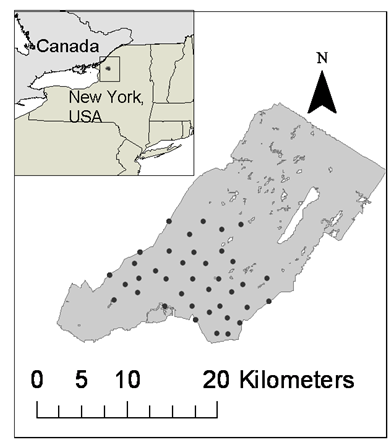
\includegraphics[height=3in]{Ch1/figs/hairsnares}
\end{center}
\caption{Locations of black bear hair snares on Fort Drum.}
\label{fig.hairsnares}
\end{figure}

We regarded this data set as a standard capture-recapture data set -
an encounter history matrix with 47 rows and 8 columns with entries
$y_{ik}$, where $y_{ik}=1$ if individual $i$ was captured in sample
$k$ and $y_{ik}=0$ otherwise. There is a standard closed population
model, colloquially referred to as ``model $M_0$'' (see Chapt. \ref{chapt.closed}), which
assumes that encounter probability $p$ is constant for all individuals
and sample periods.  We fitted model $M_0$ to the Fort Drum data using
traditional likelihood methods, yielding the maximum likelihood
estimate (MLE) of $\hat{N} = 49.19$ with an asymptotic standard error
(SE) of $1.9$.

The key issue in using closed population models with such data is how
on earth do we interpret this estimate of $N=49.19$ bears? Does it
represent the entire population of Fort Drum? Certainly not -- the trapping array covers less than
half of Fort Drum! (Fig. \ref{fig.hairsnares}). So to get at the total bear
population size of Fort Drum, we'd have to convert our $\hat{N}$ to
an estimate of density and extrapolate. To get at density, then,
should we
assert that $N$ applies to the southern half of Fort Drum below some
arbitrary line? Surely bears move on and off of Fort Drum without
regard to hypothetical boundaries. Without additional information
there is simply no way of converting this estimate of $N$ to density,
and hence it is really not meaningful biologically. To resolve this
problem, we will adopt the customary approach of converting $N$ to $D$
by buffering the convex hull around the trap array. The convex hull
has area $157.135$ $km^2$. We follow \citet{bales_etal:2005} in
buffering the convex hull of the trap array by the radius of the mean
female home range size.


%%%%\footnote{Did Bales et al. actually do this?}.
%HERE IS WHAT BALES DID:  First, we created a 95% minimum convex polygon
%for all radiolocations of adult females used in homerange
%analyses (Figure 1). Second,we buffered the
%100% minimum convex polygon for trapping locations
%with the approximate radius of the average
%95% minimum convex polygon home range of adult
%females (n = 13) using ArcView (ESRI, Redlands,
%Calif.).


The mean female home range radius was
estimated \citep{wegan:2008} for our study region to be $2.19$
km,
%\footnote{Is this number right out of Wegan's disseration?}
% YES, this is straight out of his thesis.
and
the area of the convex hull buffered by $2.19$ km is $277.01$
km$^2$. ({\bf R}
commands to compute the convex hull, buffer it, and compute the area
are given in the {\bf R} package \mbox{scrbook} which accompanies the
book).  Hence, the estimated density
here is approximately $0.178$ bears/km$^2$ for an estimated population
size obtained using model $M_0$.  We could assert that the problem has
been solved, go home, and have a beer.  But then, on the other hand,
maybe we should question the use of the estimated home range radius
 -- after all, this is only the female home range radius and the home ranges
 change for many reasons. Instead, we may decide to rely on a buffer width based on
one-half MMDM estimated from the actual hair snare data as is more customary
\citep{dice:1938}. In that case the buffer width is $1.19$ km, and the
resulting estimated density is increased to $0.225$ bears/ha$^2$ about
27 \% larger.  But wait - some studies actually found the full MMDM
\citep{parmenter_etal:2003} to be a more appropriate measure of
movement (e.g \citet{soisalo_cavalcanti:2006}). So maybe we should use
the full MMDM
which is $2.37$ km, pretty close to the telemetry-based estimate
and therefore providing a similar estimate of density ($0.171$
bears/ha$^2$). So in trying to decide how to buffer our trap array we
have already generated 3 density estimates. The crux of the matter is
obvious: Although it is intuitive that $N$ should scale with area --
the number of bears should go up as area increases and go down as area
decreases -- in this ad hoc approach of accounting for animal movement
$N$ remains the same, no matter what area we decide we sampled. The
number of bears and the area they live in are not formally tied
together within the model, because estimating $N$ and estimating the
area $N$ refers to are two completely independent analytical steps which are unrelated to one another by a
formal model.

Unfortunately, our problems don't end here. In thinking about the use of model $M_0$, we might naturally question
some of the basic assumptions that go into that model. The obvious one
to question is that which declares that $p$ is constant. One obvious
source of variation in $p$ is variation {\it among individuals}. We
expect that individuals may have more or less exposure to trapping due
to their location relative to traps, and so we try to model this ``heterogeneous''
encounter probability
phenomenon.
To illustrate this here are the number of traps that each individual was captured in:
\begin{verbatim}
 #traps:  1   2  3  4  5  6  9
 #bears: 23  13  6  2  1  1  1
\end{verbatim}
suggesting quite a range in traps exposed to by different bears.
%%% #bears: 19 15  5  2  2  1  1  1  1
% But, being captured in different numbers of traps is {\it not} inconsistent with a non-spatial model.
%That is if individuals roamed randomly over space with no ``home range'' then you should expect them to be captured
%in varying numbers of traps also.....
This has led many to consider
capture-recapture models that allow for individual heterogeneity in
$p$. Such models have the colloquial name of ``model $M_h$.''
We fitted this model (see Chapt. \ref{chapt.closed} for details) to the Fort Drum data
using each of the 3 buffer widths previously described (telemetry, 1/2
MMDM and MMDM), producing the estimates reported in Table
\ref{intro.tab.fdests}. While we can tell by the models' AIC that $M_h$ is
clearly favored by more than 30 units, we might still not be entirely
happy with our results. Clearly there is information in our data that
could tell us something about the exposure of individual bears to the
trap array -- where they were captured, and how many times -- but
since space has no representation in our model, we can't make use of
this information. Model Mh thus merely accounts for what we observe in
our data (some bears were more frequently captured than others) rather
than explicitly accounting for the processes that generated the data.

So what are we left with?  Our density estimates span  a range
from $0.17$ to $0.43$ bears/km$^2$ depending on which estimator of $N$ we use and
what buffer strip we apply. Should we feel strongly about one or the other?
Which buffer should we prefer?
AIC favors model $M_h$, but did it adequately account for the differences in
exposure of individuals to the trap array? Are we happy with a purely phenomenological model
for heterogeneity? One that posits that all bears are $iid$ draws from some distribution?
It assumes that all individuals are iid draws from some distribution but does not
account for the explicit mechanism of induced heterogeneity. And, further, we have information
about that (trap of capture) which model Mh ignores.
%Moreover, we could find more variations of
%model Mh to choose among, but see \citep{link:2003}.
And if we choose one type of buffer, how do we compare our density estimates
to those from other studies that may opt for a different kind of buffer?
The fact that $N$ doesn't scale with $A$, as part of the model, renders this choice
arbitrary. The buffer isn't part of the model.
\begin{comment} So
how do we characterize uncertainty of the buffer ``estimate''?  And,
in what sense is the
buffer even an estimate of something? What is it an estimate of?
\end{comment}
Clearly,
there is not a compelling solution to be derived from
this ``estimate $N$ and conjure up a buffer'' approach
and we are left not much wiser about bear density at
Fort Drum than we were before we conducted this analysis.

%%%% We could just finish this part off with a paragraph about these additional open questions -
%%%%the whipped cream of problems on the capture-recapture sundae - including the trap-level covariates;
%%%%or we could come up with some trap-level covariate example for the bears (different baits used, blabla).
\begin{comment}
Some of the open questions at this point:
How do we characterize uncertainty of the buffer ``estimate''?  And,
in what sense is the
buffer even an estimate of something? What is it an estimate of?
The summary here should be that there's not a compelling solution to be derived from
this ``estimate $N$ conjure up a buffer'' approach.
{\bf The main point that N doesn't scale with A is not made
  clearly here.}
\end{comment}


\begin{table}[ht]
\centering
\caption{Table on estimates of D for the Fort Drum data
using models $M_0$ and $M_h$ and different buffers. Model $M_h$ here
is a logit-normal mixture \citep{coull_agresti:1999}.}
\begin{tabular}{ll|cc}
\hline
model & buffer &  $\hat{D}$ & SE \\ \hline
M0   & telemetry &  0.178 & 0.178 \\
M0    & MMDM     &  0.171 & 0.171\\
M0   & 1/2 MMDM  &  0.225 & 0.225\\
Mh(ln) & telemetry &0.341 & 0.144\\
Mh(ln) & MMDM    &  0.327 & 0.138\\
Mh(ln) & 1/2 MMDM & 0.432 & 0.183\\
\end{tabular}
\label{intro.tab.fdests}
\end{table}


\section{Extension of Closed Population Models}
XXX Spatial context of populations ?? XXXXXX


The deficiency with classical closed population models is that they
have no spatial context. $N$ is just an integer parameter that applies
equally well to some population that exists in a computer, estimating the number
of unique words in a book, or a bucket full of goldfish.  The question
of {\it where} the $N$ items belong is central both to interpretation
of data and estimates from all capture-recapture studies and, in fact,
to the construction of spatial capture-recapture models considered in
this book.  Surely it must matter whether the $N$ items exist as words
in a book, or goldfish in a bowl, or birds in a forest patch! That
classical closed population models have no spatial context leads to a
number of conceptual and methodological problems or limitations as we
have discussed and even encountered in our analyses so far.

Thus, the essential problem is that classical closed population models
are too simple - they ignore the spatial attribution of traps and
encounter events, movement and variability in exposure of individuals
to trap proximity, and, because ordinary closed population models
possess no notion of ``area'',  they do not yield estimates of {\it density}.
These are not problems per se but rather just features
of an overly-simple class of models, and they should 
 be addressed formally by the development of
more general models.



\subsection{The modern age}

%Spatial capture-recapture models are
%statistical and mathematical models that extend non-spatial
%``ordinary'' capture-recapture models to accommodate the spatial
%structure inherent in sampling animal populations - i.e., trap
%locations, individual locations, and individual use of space.

The solution to the various issues that arise in the application of
ordinary capture-recapture models is to extend the closed population
model so that $N$ becomes spatially explicit.
%A natural way is to
%define a point process \citep{efford:2004} that describes how
%individuals are organized in space and that, when points are
%aggregated over space, the value $N$ is derived in a meaningful way.
%Thus, in this book, we adopt the view that the locations of the $N$
%individuals in the population are a {\it realization of a spatial
%  point process}.
\citet{efford:2004} was the first to formalize an explicit model for
spatial capture-recapture problems in the context of trapping arrays.
He adopted a Poisson point process model to describe the distribution
of individuals and then what is essentially a distance sampling
formulation of the observation model which describes the probability
of detection as a function of individual location, regarded as a
latent variable governed by the point process model. While earlier
(and contemporary) methods of estimating density from trap arrays have
been ad hoc in the sense of lacking a formal description of the
spatial model, Efford achieved a formalization of the model,
describing explicit mechanisms governing the spatial distribution of
individuals and how they are encountered by traps, but
adopted a more or less ad hoc framework for inference under that
spatial model using a simulation based method known as inverse
prediction \citep{gopalaswamy:2012}.

Recently, there has been a flurry of effort devoted to formalizing
inference under this model-based framework for the analysis of spatial
capture-recapture data \citep{royle_gardner:2011,borchers:2011,gopalaswamy:2012}.
There are two distinct lines of work which
adopt the model-based formulation in terms of the underlying point
process but differ primarily by the manner in which inference is
achieved. One approach \citep{borchers_efford:2008} is a classical inference approach based on
likelihood (see Chapt. \ref{chapt.mle}), and the other \citep{royle_young:2008} adopts a
Bayesian framework for inference (Chapts. \ref{chapt.scr0,chapt.mcmc}).

To motivate the origins and relevance of these approaches, we note
that, fundamentally, spatial capture-recapture models are related to
classical ``individual covariate'' models (colloquially referred to as
Huggins-Alho models) in capture-recapture \citep{huggins:1989,
  alho:1990}.  In particular, the individual covariate\footnote{have
  we mentioned what the individual covariate is, yet?} is observed in
these classical individual covariate models whereas it is not directly
observed in SCR models.  To accommodate that, a prior distribution for
the individual covariate is required.
%In essence then, SCR models are
%similar to a fully model-based formulation of classical Huggins-Alho
%models (see \citet{royle:2009}).
Likelihood analysis
\citep{borchers_efford:2008} proceeds by removing the random effect
from the likelihood by integration whereas Bayesian analysis
\citep{royle_young:2008} proceeds by analyzing the conditional model
directly, usually by methods of Markov chain Monte Carlo (MCMC).




\subsection{Abundance as the Aggregation of a Point Process}

Spatial point process models represent a major methodological theme in
spatial statistics \citep[][ch. xyz]{cressie:1992} and they are
widely applied as models for many ecological phenomena
\citep{stoyan_penttinen:2000,illian_etal:2008}. Point process models apply to
situations in which the random variable in question represents the
locations of events or objects: trees in a forest, weeds in a field,
bird nests, etc.  As such, it seems natural to describe the
organization of individuals in space using point process models. SCR models represent the
extension of ordinary capture-recapture models by augmenting the model with a point process
model to describe individual locations.

One
of the key features of SCR models is that the point locations are
latent, or unobserved, and we only obtain imperfect information about
the point locations by observing individuals at trap or observation
locations.  Thus, the realized locations of individuals represent a
type of ``thinned'' point process, where the thinning mechanism is not
random but, rather, biased by the observation mechanism.  It is
natural to think about the observed point process as some kind of a
compound or aggregate point process with a set of ``parent'' nodes
being the locations of individual home ranges or their centroids,
and the observed locations as
``offspring'' - i.e., a Poisson cluster process (PCP). In that
context, density estimation in SCR models is analogous to estimating the number of
parents of a Poisson cluster process \citep{chandler_royle:2012}.
% Other types of point
% process models for the realized locations have direct relevance to SCR
% models (See \citet{chandler_royle:2012}, discussed in chapter XYZ).

In the context of SCR models, we suppose there is a point on the
landscape that we'll think of as a home range center or, if this is
unappealing, we can think of it as the centroid of an individual's
activities during the time of sampling. In general, this point is
unknown for any individual but if we could track an individual over
time and take many observations then we could perhaps get a good idea
of where that point is.  We'll think of the collection of these points
as defining the spatial distribution of individuals in the
population. Most of the recent developments in modeling and inference
from spatial encounter history data, including most methods discussed
in this book, are predicated on the view that individuals are
organized in space according to a relatively simple point process
model. More specifically, we assume that the collection of individual
activity centers are ``$iid$'' random variables distributed uniformly
over some region. This is consistent with the assumption that the
activity centers represent the realization of a Poisson point process
or, if the total number of activity centers if fixed, then this is
usually referred to as a binomial point process.

%%I think we could shorten the home range paragraph; I like the definition
%%'the centroid of an individual's
%%% activities during the time of sampling'. I think the definition of
%% home range is something like the colleciton of points/sites/areas
%% an animal uses over the course of its lifetime so it's vague anyway
%% and what that definition means for the different forms of home
%%ranges - territory, migratory species etc - is pretty much left open.
We use the terms home range or activity center interchangeably. The
term ``home range center'' suggests that models are only relevant to
animals that exhibit such behavior of establishing home ranges or
territories and since not all species do that, perhaps the
construction of SCR models based on this idea is flawed. However,
 the notion of a home range center is just a conceptual
device and we don't view this concept as being strictly consistent
with classical notions of animal territories. Rather our view is
that a home range or territory is inherently dynamic, temporally, and thus it is a
transient quantity - where the animal lived during the period of
study,
a concept that is completely analogous to the
more conventional notion of utilization
distributions.
Therefore, whether or not individuals of a species establish home ranges
is irrelevant because, once a precise time period is defined, this defines a distinct region of space
that an individual must have occupied. In other
words, the definition of ``home range center'' is predicated
 on the specification of a time period over which individuals
are studied. A term that might be less offensive than ``home range
center'' is ``centroid of space usage (CSU)''
 which should not
conflict directly with preconceived understandings and interpretations
of home range.


\subsection{The state-space}

If we let ${\bf s}_{i}; i=1,2,\ldots,N$ be the locations of individual
activity centers, then the question ``what are the possible values of
${\bf s}$?'' needs to be addressed because the individual ${\bf
  s}_{i}$ are {\it unknown}. As a technical matter, we will regard
them as random effects and in order to apply standard methods of
statistical inference we need to provide a distribution for these
random effects.  In the context of the point process model, the
possible values of the point locations referred to as the
``state-space'' of the point process and this is some region or set of
points which we will denote by ${\cal S}$.
${\cal S}$ is a region within which points are located - essentially a
prior distribution for ${\bf s}_{i}$ (or, equivalently, the random effects
distribution).
%%Don't think prior has come up yet; maybe not that important here?
In animal studies as a description of
where individuals that could be captured are located it encloses our
study area -- the region within which we might have located traps or
detection devices.  The state-space of the point process should
accommodate all individuals that could have been captured in the study
area.

In the practical application of SCR models, in most cases estimates of
density will be relatively insensitive to choice of state-space
%%% I also think the rest of this paragraph could be postponed to a later chapter
unless there are meaningful features to the state-space
which should be accommodated. For example, if the region within which
traps are located contains a coastline or a huge body of water then
clipping that out of the state-space will typically have an
effect on density
(see
sec. \ref{scr0.sec.wolverine} for an illustration).
This should be expected because, insofar as the
state-space serves as a prior distribution on the latent variables
${\bf s}_{i}$ then, {\it the state-space is a
  component of the model. } We discuss choosing the state-space in
Chapt. \ref{chapt.scr0}.

When the underlying point process is well-defined, including a precise
definition of the state-space, this in turn induces a precise
definition of the parameter $N$ ``population size'' as the number of
individual activity centers located within the prescribed state-space.
A deficiency with some classical methods of ``adjustment'' is they
attempted to prescribe something like a state-space - a ``sampled
area'' - except absent any precise linkage of individuals with the
state-space. SCR models formalize the linkage between individuals and
space and, in doing so, provide an explicit definition of $N$
associated with
a well-defined spatial region, and hence
density. That is, the provide a model in which $N$ scales, as part of the model, with the
size of the prescribed state-space. In a sense, the whole idea of SCR models is that by defining
this point process and its state-space ${\cal S}$, this gives context and
meaning to $N$ which can be estimated directly for that specific
state-space. Thus, it is fixing ${\cal S}$ that resolves the problem of
``unknown area'' that we have previously discussed.
\begin{comment}
%% I find the next two sentences a little confusing
But the
existence of an explicit state-space ${\cal S}$ is kind of beside the
point -- ${\cal S}$ is really not always terribly important
itself. Instead, as soon as you give the latent variables ${\bf s}$ a
place to live, and this is recognized explicitly in the model upon which inference is based,
 then you achieve spatial explicitness of the model.
\end{comment}



\section{Elements of SCR Models}

The state-space of the latent point process is the critical element of SCR models but there
are many more aspects relevant to the formulation of SCR models for specific situations.
We address some of these in more detail in the following chapter....

Broadly speaking we differentiate
between two situations: Sampling based on fixed arrays or sampling
based on ``search encounter'' methods. The former includes things like
camera traps, hair snares, mist nets and conventional traps. Fixed
arrays limit the observation location to pre-defined points, where
traps are located. Using such methods the model is a little simpler
because the ``movement process'' of individuals is confounded with the
``observation process''.
The 2nd type of model -- search encounter models -- typically
will allow locations in continuous space, possibly only restricted by
polygon boundaries \citep{royle_young:2008}.
Search-encounter data
usually allow for the separate modeling and estimation of movement
model parameters from encounter model parameters but not always,
depending on whether replication of the sampling is done.  The
classical distance sampling model with no replication (i.e., $t=1$) is a basic model
which confounds the two processes.


Depending on the type of device being considered, certain restrictions
on the observable variable are induced which suggest specific
probability models for the observable random variable, suggesting
either binomial, Poisson or multinomial (and possibly other)
observation models.
One type of a
device is what we think of as the classical ``camera trap'' and which
\citet{efford:2011} refers to as a ``proximity detector''. We can take
pictures of or detect any number of individuals and an individual can
be caught in any number of traps, and an arbitrary number of
times. Iid Bernoulli model is convenient but if you think the
re-encounters are valuable then you can have a frequency model.  Bear
hair snares are slightly different because you cannot differentiate
re-encounters.
The standard observation model that applies for ``single-catch''
\citep{efford_etal:2004} traps posits that individuals are encountered
in at most one trap per sample occasion and traps only hold one
individual.  Unfortunately we're really screwed in the single-catch
situation.
A ``multi-catch'' is like a mist-net or other things - individual is
captured and restrained but traps hold > 1 individual. In this case,
the observation model is a multinomial. There are
many variations on all of these models and new models.







\begin{comment}

\subsection{Why is density so important? }

Knowledge of population size is a fundamental piece of information in
conservation. Since the risk of a species/population going extinct is
a function of how many individuals of that species there are, much of
conservation-related research revolves around abundance. Consider, for
example, the concept of minimum viable population size � to assess
whether a population has a good chance of persistence over some time
frame we need to know how big it is to begin with. The idea of a
minimum viable population is reflected in many applied conservation
efforts. For example, in a range-wide assessment of the jaguar�s
population status, researchers were asked to delineate Jaguar
Conservation Units (JCU�s), of which one criterion was ``holding at
least 50 jaguars'' � a number considered a substantial population
\citep{sanderson_etal:2002}.

While the importance of abundance is indisputable, there are some
major issues associated with this measure. First, you cannot compare
mere values of abundance unless they refer to a specific area. If you
look at the IUCN Red List of Endangered Species entry for the
population status of the tiger, it will tell you that there are an
estimated 1700 tigers in India but only about 20 in Cambodia
\citep{chundawat_etal:2011}. Now, this will not automatically make you
lament the state of tiger conservation in Cambodia as compared to
India (although seeing these numbers you might well lament the state
of the tiger in general), because you know these numbers refer to
countries that are extremely different in size. Rather, if you wanted
to know something about where tigers are currently doing better,
you�d probably divide the number of tigers by the countries�
areas and compare tiger densities (turns out India�s tigers are
still doing better, not by a factor of 85, as mere abundances suggest,
but by a factor of 5). Although abundance and density are obviously
directly related to each other, they are different in their
applicability. Particularly, density as a scaled measure lets us
compare results across sites (as we just demonstrated for the tiger
example). In addition, some concepts incorporated in conservation
biology explicitly deal with density. For example, population growth
rate, home ranges or the probability of epidemics/disease spread are
density-dependent; the Allee effect links individual reproductive
success to population density in low-density populations.

Second, going back to the tiger example once more, we may wonder how
researchers even came up with these numbers for total population
size. Tiger abundance can be estimated using camera-traps, because
individuals have distinct stripe patterns so that photographic data
can be analyzed with capture-recapture models. But surely, no-one ever
camera-trapped the whole of India. This is a typical situation, even
on a much smaller scale. Ecologists generally sample only a small
fraction of the area used by a species or population, but want to
estimate total population size, i.e. the number of individuals
occurring in sampled {\it and unsampled} areas. If we can use the data
from sampled area to obtain a density estimate, explicit predictions
of abundance can be made to regions of any size (assuming that density
is constant across the region we are inferring to and equal to density
in the sampled area)\footnote{Note that the way total tiger abundance
  estimates are derived for India is much more complex than just
  looking at tiger density somewhere in India and then extrapolating
  it to the entire country (for details, see \citep{jhala_etal:2011});
  we merely use these numbers here to illustrate the general
  problem.}.

To summarize, density not only influences several ecological
processes, but also allows us to compare population status among
different sites; even where total abundance is of primary interest,
density can help us arrive at a total population estimate even when
we�re unable to survey the total population. Capture-recapture
models were designed to estimate abundance, but they generally cannot
be used to formally estimate density. This limitation of non-spatial
CR models has long been recognized (REF) and several ad hoc approaches
to overcome this problem have been devised. We will discuss those and
their shortcomings in XXX. The great advantage of SCR models over
non-spatial capture-recapture models is that they formally link
abundance and area so that they actually estimate density.


\end{comment}









\section{Summary and Outlook}


Spatial capture-recapture models are an extension of ordinary
capture-recapture models to accommodate the spatial organization of
both individuals in a population and the observation mechanism (e.g.,
locations of traps).  They resolve problems which have been recognized
historically and for which various ad hoc solutions have been
suggested: heterogeneity in encounter probability due to the spatial
organization of individuals relative to traps, the need to model
trap-level effects on encounter, and that a
well-defined sample area does not exist in most studies, and thus
estimates of $N$ using ordinary capture-recapture models cannot be
related directly to density.

\subsection{The Promise of Spatial Capture-Recapture}

However, SCR models are not merely an extension of technique but
rather they represent an extention in a much more
profound way in that they make ecological processes explicit in the
model -- processes of spatial organization of individuals, movement
and space-usage of individuals. While capture-recapture models have
existed for decades this is a completely new element of
closed capture-recapture models.
This is so profoundly important because
ecological scientists study elements of ecological theory using
observational data that exhibits various biases relating to the
observation mechanisms employed. In the context of capture-recapture,
we observe individual encounter history data from which we can use SCR
models to infer where individual live, how they organize themselves in
space and move around in space and how they interact with other
individuals.  Spatial capture-recapture models show great promise in their ability
to integrate explicit ecological theories directly into the models so
that we can directly test hypotheses about either space usage (e.g.,
Chapt. \ref{chapt.ecoldist}) or movement (Chapt. \ref{chapt.searchencounter}) or the distribution of
individuals in space (Chapt. \ref{chapt.state-space}). We imagine that in the near future
SCR models will include point process models that allow for
interactions among individuals such as inhibition or  clustering (REF XXXX).

Thus, SCR models are capture-recapture models that enable ecologists
to explicitly integrate biological context and theory with encounter
history data, which is something that has always been the focus of
``open population'' models but never, until very recently, has been
considered formally in closed population models. We therefore believe
that SCR models will enable ecologists to test theories of space usage
and environmental effects, social behavior and other important
theories.


<<<<<<< HEAD
=======
\subsection{What Lies Ahead}

In the following chapters we develop a comprehensive synthesis and extension of
spatial capture-recapture models.
Roughly the first third of the book is introductory material --
In Chapt. \ref{chapt.glms} we provide the basic analysis tools to understand and
analyze SCR models - namely generalized linear models (GLMs) with random effects, and their
analysis in {\bf R} and {\bf WinBUGS}.  Because SCR models represent extensions of
basic closed population models, we cover ordinary closed population
models in Chapt. \ref{chapt.closed} wherein, along with Chapts. \ref{chapt.scr0} and \ref{chapt.poisson-mn}
\footnote{might ought to put Modeling Encounter Probability
as chapter 5 instead}, provides the basic introduction
to capture-recapture models and their spatial extension.
We will see that
SCR models are a
conceptual and technical intermediates between the class of models referred to as
model $M_h$, and so-called
individual covariate models.
We develop technical tools for likelihood (Chapt. \ref{chapt.mle})
and Bayesian analysis (Chapt. \ref{chapt.mcmc}).
The middle part of the book expands set of models that we can deal with to include alternative
observation models related to the type of encounter device (Chapt. \ref{chapt.poisson-mn}), models for encounter probability
(Chapt. \ref{chapt.covariates}), [should include search-encounter models right after Poisson-mn type models?] and provides basic tools for model fit and selection (Chapt. \ref{chapt.gof}).
[should include the design chapter right here].
Finally in the last third of the book we address more advanced stuff including modeling
space usage in the encounter process (Chapt. \ref{chapt.ecoldist}), modeling state-space covariates, covariates
that affect density, (Chapt. \ref{chapt.state-space}), open population models (Chapt. \ref{chapt.open}),
models that include unmarked individuals either entirely (Chapt. \ref{chapt.scr-unmarked})
or partially marked samples (Chapt. \ref{chapt.partialID}).

In Chapter XXXX We cover a mish-mash of ideas: using telemetry data, multiple encounter methods, alternative
point-process models, and other topics that are useful but that are not fully developed or that we don't have
room for in this book.





>>>>>>> a4f454ca316a5c34e0c913aa75c0dd27a11e84c7

\chapter{Introduction}
\label{chapt.intro}

\chapter{GLMS and WinBUGS}
\label{chapt.glms}

\chapter{Closed population models}
\label{chapt.closed}

\chapter{Fully Spatial capture-recapture models}
\label{chapt.scr0}

\chapter{Other observation models}
\label{chapt.poisson}



a\chapter{
Likelihood Analysis of Spatial Capture-Recapture Models
}
\markboth{Chapter 5}{}
\label{chapt.mle}

%%%% TO-DO LIST
% 1. comparison of Bayes with MLE for wolverine data (need to rerun WinBUGS)
% 2. Beth clean up a couple things in SECR analysis.
% 3. Need to finish MLE for restricted state-space
%%   requires code from Rahel
% 4. draft up intlik3 wrapper "scr()"

\vspace{.3in}



In this book we mainly focus on Bayesian analysis of spatial
capture-recapture models. And, in the previous chapters we learned how
to fit some basic spatial capture-recapture models using a Bayesian
formulation of the models analyzed in BUGS engines including {\bf
  WinBUGS} and {\bf JAGS}.  Despite our focus on Bayesian analysis, it
is instructive to develop the basic conceptual and methodological
ideas behind classical analysis based on likelihood methods and
frequentist inference.  
This has been the approach taken by
\citet{borchers_efford:2008, dawson_efford:2009} and related papers.
Simple SCR models can be analyzed
fairly easily using such methods and, including even some classes of
models that we have not been able to fit using Bayesian methods. One
such class of models are those
that account for ecological distance in the detection model,
which we cover in  Chapt. \ref{chapt.ecoldist}).


This chapter provides some conceptual and technical footing for
likelihood-based analysis of spatial capture-recapture models. We
recognized earlier (Chapt. 4) that SCR models are versions of
binomial (or other) GLMs, but with random effects – i.e., GLMMs. These
models are 
routinely analyzed by likelihood methods. In particular, likelihood
analysis is based on the integrated likelihood in which the random
effects are removed by integration from the likelihood. In SCR models,
the random effect, ${\bf s}$, i.e., the 2-dimensional coordinate, is a
bivariate random effect. 

In this chapter, we show that it is
straightforward to compute the maximum likelihood estimates (MLE) for
SCR models by integrated likelihood. We develop the MLE framework
using {\bf R}, and we also provide a basic introduction to an {\bf R} package
\mbox{\tt secr} \citep{efford:2011} which is based on the stand-alone
package 
{\bf DENSITY} \citep{efford_etal:2004}.
 To set the context we analyze the SCR model
here when $N$ is known because, in that case, it is precisely a GLMM and
does not pose any difficulty at all. We generalize the model to allow
for unknown $N$ using both conventional ideas based on the ``joint
likelihood'' \citep[e.g.,][]{borchers_etal:2002}
and also using a formulation
based on data augmentation.  We obtain the MLEs for 
the SCR model from the wolverine camera trapping study \citep{magoun_etal:2011}
 analyzed in previous chapters to compare/contrast the
results.

\section{Likelihood analysis }

We noted in chapter 4 that, with $N$ known, the basic SCR model is a
type of binomial regression with a random effect. For such models we
can easily obtain maximum likelihood estimators of model parameters
based on integrated likelihood. The integrated likelihood is based on
the marginal distribution of the data $y$ in which the random effects
are removed by integration. Conceptually, our model is a specification
of the conditional-on-${\bf s}$ model $[y|{\bf s},\alpha]$ and we have
a ``prior distribution'' for ${\bf s}$, say $[{\bf s}]$, and the
marginal distribution of the data $y$ is
\[
[y|\alpha] =  \int_{\bf s} [y|{\bf s},\alpha][{\bf s}] d{\bf s}.
\]
When viewed as a function of $\alpha$ for pursposes of estimation, the
marginal distribution $[y|\alpha]$ is often referred to as the {\it
  integrated likelihood}.

It is worth analyzing 
the simplest SCR model with known-$N$ in order to understand the
underlying mechanics and basic concepts. These are directly relevant to
the manner in which many capture-recapture models are classically
analyzed, such as model $M_h$, and individual covariate models (see
chapt. \ref{chapt.closed} and  \citet[][chapt. 6]{royle_dorazio:2008}). To develop integrated
likelihood for SCR models, we first identify the conditional
likelhiood. 

The observation model for each encounter observation $y_{ij}$,
specified conditional on ${\bf s}_{i}$, is 
\begin{equation}
	y_{ij}| {\bf s}_{i} \sim \mbox{Bin}(K, p_{\alpha}({\bf x}_{j},{\bf s}_{i}))
\label{mle.eq.cond-on-s}
\end{equation}
where we have indicated the dependence of $p_{ij}$ on ${\bf s}$ and
parameters $\alpha$
explicitly.
For the random effect we have ${\bf s}_{i} \sim  \mbox{Unif}({\cal
  S})$.
The joint distribution of the data for individual $i$ is the product
of $J$ such terms (i.e., contributions from each of $J$ traps).
\[
  [{\bf y}_{i} | {\bf s}_{i} , \alpha] = 
  \prod_{j=1}^{J} \mbox{Bin}(K, p_{\alpha}({\bf x}_{j},{\bf s}_{i}) )
\]
We note this assumes that encounter of individual $i$ in each
trap is independent of encounter in every other trap, conditional on
${\bf s}_{i}$, this is the fundamental property of the basic model SCR0.


 The so-called marginal likelihood is computed by removing
${\bf s}_{i}$, by integration (hence also {\it integrated} likelihood), from the conditional-on-${\bf s}$
likelihood and regarding the {\it marginal} distribution of the data
as 
the likelihood. That
is, we compute:
\[
  [y|\alpha] = 
\int_{{\cal S}}  [ {\bf y}_{i} |{\bf s}_{i}, \alpha] g({\bf s}_{i}) d{\bf s}_{i}
\]
In most SCR models, $g({\bf s}) = 1/||{\cal S}||$ (but see Chapt. \ref{chapt.state-space}).

The joint likelihood for all $N$ individuals, assuming independence of
encounters among individuals, is the product of $N$ such terms:
\[
{\cal L}(\alpha | {\bf y}_{1},{\bf y}_{2},\ldots, {\bf y}_{N}) =     \prod_{i=1}^{N}
[{\bf y}_{i}|\alpha]
\]
We emphasize that two independence assumptions are explicit in this
development: independence of trap-specific encounters within
individuals and also independence among individuals. In particular,
this would only be valid when individuals are not physically
restrained or removed upon capture, and when traps do not ``fill up''.

The key operation for computing the likelihood is solving a
2-dimensional integration problem. There are some general purpose {\bf
  R} packages that implement a number of 
 multi-dimensional integration routines
including \mbox{\tt adapt} \citep{genz_etal:2007} and \mbox{\tt R2cuba}
\citep{hahn_etal:2011}.  In practice, we won't rely
on these extraneous {\bf R} packages (except see
chapt. \ref{chapt.state-space} for an application of \mbox{\tt Rcuba})
but instead will use perhaps less
efficient methods in which we replace the integral with a summation
over an equal area mesh of points on the state-space ${\cal S}$ and explicitly
evaluate the integrand at each point. We invoke the rectangular rule
for integration here\footnote{e.g., 
\url{http://en.wikipedia.org/wiki/Rectangle_method}
} in which we
evaluate the
integrand on a regular grid of points of equal area and compute the
average of
the integrand over that grid of points. 
Let $u=1,2,\ldots,nG$ index a grid of
$nG$ points, ${\bf s}_{u}$,  where the area of grid cell $u$ is
constant, say $A$.
In this case, the integrand, i.e., the marginal pmf of 
${\bf y}_{i}$, is approximated by  
\begin{equation}
         [{\bf y}_{i}|\alpha] = \frac{1}{nG} \sum_{u=1}^{nG}  [ {\bf
            y}_{i} |{\bf s}_u, \alpha]
\label{mle.eq.intlik}
\end{equation}

This is a specific case of the general expression that could be used
for approximating the integral for any arbitrary (bivariate or otherwise)
distribution $g({\bf s})$. The general case is
\[
[y]  = \frac{A}{nG} \sum_{u} [y|{\bf s}_{u}] [{\bf s}_{u}]
\]
 In the present context it happens that  $[{\bf s}] = (1/A)$
and thus the grid-cell area cancels in the above
expression to yield eq. \ref{mle.eq.intlik}.
The rectangular rule for integration can be seen as an application of
the Law of Total Probability for a discrete random variable ${\bf
  s}$, having $nG$ 
unique values with equal probabilities $1/nG$.



\subsection{ Implementation (simulated data)}

Here we will illustrate how to carryout this integration and
optimization based on the integrated likelihood using simulated data
 (i.e., following that from Chapter 4). Using \mbox{\tt simSCR0.fn}
 we simulate data for 100 individuals and a 25 trap array
layed out in a $5 \times 5$ grid of unit spacing.  The specific encounter
model is the half-normal model. The 100 activity centers were
simulated on a state-space defined by a $8 \times 8$ square 
within which the
trap array was centered (thus the trap array is buffered by 2
units). Therefore, the density of individuals in this system is fixed
at $100/64$.

In the following set of {\bf R} commands we generate the data and 
then harvest the required data objects:
{\small
\begin{verbatim}
data<-simSCR0.fn(discard0=FALSE,sd=2013)
y<-data$Y
traplocs<-data$traplocs
nind<-nrow(y)
X<-data$traplocs
J<-nrow(X)
K<-data$K
Xl<-data$xlim[1]
Yl<-data$ylim[1]
Xu<-data$xlim[2]
Yu<-data$ylim[2]
\end{verbatim}
}
Now we need to define the integration grid, say ${\bf G}$, which we do with
the following set of {\bf R} commands (here, \mbox{\tt delta} is the grid spacing):
{\small
\begin{verbatim}
delta<- .2
xg<-seq(Xl+delta/2,Xu-delta/2,by=delta) 
yg<-seq(Yl+delta/2,Yu-delta/2,by=delta) 
npix<-length(xg)          # assumes xg and yg same dimension here
area<- (Xu-Xl)*(Yu-Yl)/((npix)*(npix)) # don’t need area for anything
G<-cbind(rep(xg,npix),sort(rep(yg,npix)))
nG<-nrow(G)
\end{verbatim}
}
In this case, the integration grid is set up as a grid with spacing
$\delta = 0.2$ which produces a $40 \times 40$ grid of points for evaluating the
integrand if the state-space buffer is set at 2.

We next create an {\bf R} function that defines the likelihood as a function
of the data objects $y$ and $X$ which were created above but, in general,
you would read these files into {\bf R}, e.g., from a .csv file.
In addition to these data
objects, we need to have defined the  quantities $G$ and $nG$ associated
with the integration grid.
However, instead of worrying about making all of these objects and
keeping track of them we just put that code above into the likelihood
function, say \mbox{\tt intlik1}, and pass $\delta$ as an additional (optional) argument and a
few other things that we need such as the boundary of the state-space
over which the integration (summation) is being done. This function is
available in the package \mbox{\tt scrbook}, and it is reproduced here:

{\small 
\begin{verbatim}
intlik1<-function(parm,y=y,delta=.2,X=traplocs,ssbuffer=2){

Xl<-min(X[,1]) - ssbuffer 
Xu<-max(X[,1]) + ssbuffer
Yu<-max(X[,2]) + ssbuffer
Yl<-min(X[,2]) - ssbuffer

xg<-seq(Xl+delta/2,Xu-delta/2,,length=npix) 
yg<-seq(Yl+delta/2,Yu-delta/2,,length=npix) 
npix<-length(xg)

G<-cbind(rep(xg,npix),sort(rep(yg,npix)))
nG<-nrow(G)
D<- e2dist(X,G)  

alpha0<-parm[1]
alpha1<-parm[2]
probcap<- plogis(alpha0)*exp(-alpha1*D*D)
Pm<-matrix(NA,nrow=nrow(probcap),ncol=ncol(probcap))
                    # all zero encounter histories
n0<-sum(apply(y,1,sum)==0) 
                    # encounter histories with at least 1 detection
ymat<-y[apply(y,1,sum)>0,] 
ymat<-rbind(ymat,rep(0,ncol(ymat)))
lik.marg<-rep(NA,nrow(ymat))
for(i in 1:nrow(ymat)){
Pm[1:length(Pm)]<- (dbinom(rep(ymat[i,],nG),K,probcap[1:length(Pm)],log=TRUE))
lik.cond<- exp(colSums(Pm))
lik.marg[i]<- sum( lik.cond*(1/nG))  
}
nv<-c(rep(1,length(lik.marg)-1),n0)
-1*( sum(nv*log(lik.marg)) )
}
\end{verbatim}
}


The function accepts as
input the encounter history matrix, $y$, the trap locations, $X$, and the
state-space buffer. This allows us to vary the state-space buffer and
easily evaluate the sensitivity of the MLE to the size of the
state-space. 
Note that we have a peculiar handling of the encounter history
matrix $y$. In particular, we remove the all-zero encounter histories
from the matrix and tack-on a single all-zero encounter history as the
last row which then gets weighted by the number of such encounter
histories (\mbox{\tt n0}). This is a bit long-winded and strictly unnecessary
when $N$ is known, but we did it this way because the extension to the
unknown-$N$ case is now transparent (as we demonstrate in the following
section). 
 The matrix \mbox{\tt Pm} holds the log-likelihood contributions of
each encounter frequency for each possible state-space location of the
individual. 
The log contributions are summed up and the result
exponentiated on the next line, producing lik.cond, the
conditional-on-${\bf s}$ likelihood (Eq. \ref{mle.eq.cond-on-s}
above). The marginal
likelihood (\mbox{\tt lik.marg}) sums up the conditional elements weighted by
$\Pr({\bf s})$ (Eq. \ref{mle.eq.intlik} above).
This is a fairly primative function which doesn't allow much
flexibility in the data structure. For example, it assumes that $K$,
the number 
of replicates, is constant for each trap. Further, it assumes that the
state-space is a square. We generalize this to some extent later in
this chapter. 

Here is the {\bf R} command for maximizing the likelihood and saving the
results into an object called \mbox{\tt frog}.  The output is a list of the
following structure and these specific estimates are produced using
the simulated data set:

{\small 
\begin{verbatim}
# should take 15-30 seconds

starts<-c(-2,2)
frog<-nlm(intlik1,starts,y=y,delta=.1,X=traplocs,ssbuffer=2,hessian=TRUE)
frog

$minimum
[1] 297.1896

$estimate
[1] -2.504824  2.373343

$gradient
[1] -2.069654e-05  1.968754e-05

$hessian
          [,1]      [,2]
[1,]  48.67898 -19.25750
[2,] -19.25750  13.34114

$code
[1] 1

$iterations
[1] 11
\end{verbatim}
} 
Details about this output can be found on the help page for
\mbox{\tt nlm}. We note briefly that \mbox{\tt frog\$minimum} is the
negative log-likelihood value at the MLEs, which are stored in the
\mbox{\tt frog\$estimate} component of the list. The hessian is the
observed Fisher information matrix, which can be inverted to obtain
the variance-covariance matrix using the commands:
\begin{verbatim}
> solve(frog$hessian)
\end{verbatim}

It is worth drawing attention to the fact that the estimates are
different than the Bayesian estimates reported previously in Chapt. \ref{chapt.scr0}.
How can that be?!  There are several reasons for
this.  First Bayesian inference is based on the posterior distribution
and it is not generally the case that the MLE should correspond to any
particular value of the posterior distribution. If the prior
distributions in a Bayesian analysis are uniform, then the
(multivariate) mode of the
posterior is the MLE, but note that Bayesians almost always report
posterior {\it means} and so there will typically be a discrepancy
there. Secondly, we have implemented an approximation to the integral
here and there might be a slight bit of error induced by that. We will
evaluate that shortly. Third, the Bayesian analysis by MCMC is subject
to some amount of Monte Carlo error which the analyst should always be
aware of in practical situations.  All of these different explanations
are likely responsible for some of the discrepancy. Accounting for
these, we see general consistency between the
two estimates.

To compute the integrated likelihood we used a discrete representation
of the state-space so that the integral could be approximated as a
summation over possible values of ${\bf s}$ with each value being
weighted by its probability of occurring, which is $1/nG$ under the
assumption that ${\bf s}$ is uniform on the state-space ${\cal
  S}$. Recall
in Chapt. \ref{chapt.scr0} we 
used a discrete state-space in developing a Bayesian analysis of the
model in order to be able to modify the state-space in a flexible
manner. In that case, we could use the discretized state-space as the
integration grid and just feed it into our integrated likelihood
routine. 

In summary, we note that, for the basic SCR model, integrated
likelihood is a really easy calculation when $N$ is known. Even for $N$
unknown it is not too difficult, and we will do that shortly.
However, if you can solve the known-$N$ problem then you should be able
to do a real analysis, for example by considering different values of
$N$ and computing the results for each value and then making a plot of
the log-likelihood or AIC and choosing the value of $N$ that produces
the best log-likelihood or AIC. As a homework problem we suggest that
the reader take the code given above and try to estimate $N$ without
modifying the code – by just repeatedly calling that code for
different values of $N$ and trying to deduce the best value.
We will formalize the unknown-$N$ problem shortly.

The
software package {\bf DENSITY} \citep{efford_etal:2004} implements
certain types of SCR models using integrated likelihood methods, and
\mbox{\tt secr} \citep{efford:2011} is an {\bf R} package with similar functionality.
We provide an analysis of some data using \mbox{\tt secr} shortly along
with a discussion of its capabilities, and we use \mbox{\tt secr} in
later chapters for likelihood analysis of other SCR models.


\section{MLE when N is Unknown} 

Here we build on the previous introduction to integrated likelihood
but we consider now the case in which $N$ is unknown. We will see that
adapting the analysis based on the known-$N$ model is really
straightforward for the more general problem. The main distinction is
that we don’t observe the all-zero encounter history so we have to
make sure we compute the probability for that encounter history which
we do by tacking a row of zeros onto the encounter history matrix. In
addition, we include the number of such all-zero encounter histories
as an unknown parameter of the model. Call that unknown quantity
$n_{0}$, and we have to 
be sure to include a combinatorial term to
account for the fact that of the $n$ observed individuals there are
${N \choose n}$
 ways to realize a sample of size $n$. The combinatorial term
involves the unknown $n_{0}$ and thus it must be included in the likelihood.

Operationally then, things proceed much as before: 
We compute the marginal probability of each observed ${\bf y}_{i}$,
i.e., by removing the latent ${\bf s}_{i}$ by integration. In
addition, we 
 compute the marginal probability of the ``all-zero'' encounter
history ${\bf y}_{n+1}$, and make sure to weight it $n_{0}$ times. We
accomplish this by ``padding'' the data set with a single encounter
history having $y_{n+1,j}=0$ for all traps $j=1,2,\ldots,J$. Then we
be sure to include the combinatorial term in the likelihood or
log-likelihood computation. We demonstrate this shortly.

To analyze a specific case, we’ll read in our fake data set (simulated
using the parameters given above). To set some things up in our
workspace we do this:
\begin{verbatim}
data<-simSCR0.fn(discard0=TRUE,sd=2013)
y<-data$Y
nind<-nrow(y)
X<-data$traplocs
J<-nrow(X)
K<-data$K
\end{verbatim}
Recall that these data were generated with $N=100$, on an $8 \times 8$ unit
state-space representing the trap locations (${\bf X}$) buffered by 2 units.

As before, the likelihood is defined in the {\bf R} workspace as an
{\bf R}
function, \mbox{\tt intlik2} (contained in the package \mbox{\tt
  scrbook}),
 which takes an argument being the unknown parameters of the
model and additional arguments as prescribed. In particular, 
 we provide the encounter history matrix ${\bf y}$, the trap locations
\mbox{\tt traplocs}, the spacing of the integration grid (argument
\mbox{\tt delta}) and the
state-space buffer. Here is the new likelihood function:
{\small
\begin{verbatim}
intlik2<-function(parm,y=y,delta=.3,X=traplocs,ssbuffer=2){

Xl<-min(X[,1]) -ssbuffer
Xu<-max(X[,1])+ ssbuffer
Yu<-max(X[,2])+ ssbuffer
Yl<-min(X[,2])- ssbuffer

xg<-seq(Xl+delta/2,Xu-delta/2,delta) 
yg<-seq(Yl+delta/2,Yu-delta/2,delta) 
npix.x<-length(xg)
npix.y<-length(yg)
area<- (Xu-Xl)*(Yu-Yl)/((npix.x)*(npix.y))
G<-cbind(rep(xg,npix.y),sort(rep(yg,npix.x)))
nG<-nrow(G)
D<- e2dist(X,G) 

alpha0<-parm[1]
alpha1<-parm[2]
n0<-exp(parm[3])
probcap<- plogis(alpha0)*exp(-alpha1*D*D)
Pm<-matrix(NA,nrow=nrow(probcap),ncol=ncol(probcap))
ymat<-rbind(y,rep(0,ncol(y)))

lik.marg<-rep(NA,nrow(ymat))
for(i in 1:nrow(ymat)){
Pm[1:length(Pm)]<- (dbinom(rep(ymat[i,],nG),K,probcap[1:length(Pm)],log=TRUE))
lik.cond<- exp(colSums(Pm))
lik.marg[i]<- sum( lik.cond*(1/nG) )  
}                                                 
nv<-c(rep(1,length(lik.marg)-1),n0)
part1<- lgamma(nrow(y)+n0+1) - lgamma(n0+1)
part2<- sum(nv*log(lik.marg))
 -1*(part1+ part2)
}
\end{verbatim}
}
To execute this function for the data that we created with \mbox{\tt simSCR0.fn},
 we execute the following command (saving the result in our
friend \mbox{\tt frog}).
This results in the usual output, including the parameter estimates,
the gradient, and the numerical Hessian which is useful for obtaining
asymptotic standard errors (see below):
\begin{verbatim}
starts<-c(-2.5,2,log(4))
frog<-nlm(intlik2,starts,hessian=TRUE,y=y,X=X,delta=.2,ssbuffer=2)

There were 50 or more warnings (use warnings() to see the first 50)

frog
$minimum
[1] 113.5004

$estimate
[1] -2.538334  2.466515  4.232810

[... Additional output deleted ...]
\end{verbatim}
While this produces some {\bf R} warnings, these happen to be harmless
in this case, and we will see from the \mbox{\tt nlm} output that the
algorithm performed satisfactory in minimizing the objective function.
The estimate of population size for the state-space (using the default 
state-space buffer) is
\begin{verbatim}
nrow(y)+exp(4.2328)
[1] 110.9099
\end{verbatim}
Which differs from the data-generating value ($N=100$) as we might
expect for a single realization. We usually will present an estimate of uncertainty assocated
with this MLE which we can obtain by inverting the Hessian. Note that
$Var(\hat{N}) = n + \mbox{Var}(\hat{n}_{0})$.
Since we
have parameterized the model in terms of $log(n_{0})$ we use a delta
approximation to obtain the variance on the scale of $n_{0}$ as
follows:
\begin{verbatim}
(exp(4.2328)^2)*solve(frog$hessian)[3,3]
[1] 260.2033
> sqrt(260)
[1] 16.12452
\end{verbatim}
Therefore, the asymptotic ``Wald-type'' confidence interval for $N$ is
$110.91 \pm 1.96 \times 16.125 = (79.305, 142.515)$. To report this in
terms of density, we scale appropriately by the area of the prescribed
state-space which is $64$ units of area (i.e., an $8 \times 8$ square).


\begin{comment}

\subsection{Exercises}

{\flushleft 
{\bf 1.}	
Run the analysis with different state-space buffers and comment on the result. 
}


{\flushleft 
{\bf 2.} Conduct a brief simulation study using this code by
  simulating 100 data sets and obtain the MLEs for each data set. Do
  things seem to be working as you expect?  }

{\flushleft 
{\bf 3.} 
Further extensions: It should be straightforward to
  generalize the integrated likelihood function to accommodate many
  different situations. For examples, if we want to include more
  covariates in the model we can just add stuff to the object \mbox{\tt probcap},
 and add the relevant parameters to the argument that gets
  passed to the main  function.  For the simulated data, make up a
  covariate by generating a Bernoulli covariate (``trap type'' – perhaps
  baited or not baited) randomly and try to modify the likelihood to
  accommodate that.  }

{\flushleft {\bf 4.}  We would probably be interested in devising the
  integrated likelihood for the full 3-d encounter history array so
  that we could include temporally varying covariates. This is not
  difficult but naturally will slow down the execution
  substantially. The interested reader should try to expand the
  capabilities of this basic {\bf R} function.  }
\end{comment}




\subsection{Integrated Likelihood using the model under data augmentation } 

Note that this likelihood analysis is based on the standard likelihood
in which $N$ (or $n_{0}$) is an explicit parameter. This is usually called
the ``joint likelihood'' or ``unconditional likelihood''.  We could also
express the joint likelihood using data augmentation, replacing the
parameter $N$ with $\psi$ \citep[e.g., see Sec. 7.1.6][for an example]{royle_dorazio:2008}.
We don't go into detail here, but we note that the
likelihood under data augmentation is a zero-inflated binomial
mixture – precisely an occupancy type model \citep{royle:2006}.
Thus, while it is possible to carryout likelihood analysis of
models under data augmentation, we primarily advocate data
augmentation for Bayesian analysis.


\subsection{ Extensions}

We have only considered basic SCR models with no additional
covariates. However, in practice, we are interested in other types of
covariate effects including ``behavioral response'', 
sex-specificity of parameters, and potentially other effects. Some of
these  can be added directly to the likelihood – if the covariate is fixed
and known for all individuals captured or not. An example is a
behavioral response, which amounts to having a covariate $x_{ik}=1$ if
individual $i$ was captured prior to occasion $k$ and $x_{ik}=0$
otherwise. For uncaptured individuals, $x_{ik}=0$ for all $k$.
 \citet{royle_etal:2011jwm} called this a global behavioral
response because the covariate is defined for all traps, no matter the
trap in which an individual was captured. We could also define a {\it
  local} behavioral response which occurs at the level of the trap,
i.e., $x_{ijk}=1$ if individual $i$ was captured in trap $j$ prior to
occassion $k$, etc.. 
Trap-specific covariates such as trap type or status, or
time-specific covariates such as date, are easily accommodated as
well. As an example, \citet{kery_etal:2010} develop a model for the
European wildcat in which traps are either baited or not (a
trap-specific covariate with only 2 values), and also encounter
probability varies over time in the form of a quadratic seasonal response.
We consider models with behavioral response or fixed covariates in
Chapt. \ref{chapt.covariates}.
Although the integrated likelihood routines we provided above can be
modified directly for such cases, which we leave to the interested
reader to investigate. 

Sex-specificity is more difficult to deal with since sex is not known
for uncaptured individuals (and sometimes not even for all captured
individuals).  To analyze such models, we do Bayesian analysis of the
joint likelihood facilitated by the use of data augmentation
\citep{gardner_etal:2010jwm,russell_etal:2012}. For covariates that are
not fixed and known for all individuals, it is somewhat more
challenging to do MLE for these based on the joint likelihood as we
have developed above. Instead it is more conventional to use what is
colloquially referred to as the ``Huggins-Alho'' type model which is
one of the approaches taken in the software package \mbox{\tt secr}
\citep[][see Sec. \ref{mle.sec.secr}]{efford:2011}. This idea is
motivated by thinking about unequal probability sampling methods known
as Horvitz-Thompson sampling \citep[e.g.,
see][]{overton_stehman:1995}.  We don't use that method anywhere in
this book because it represents a paradigm shift in the inference
framework which is done historically only for convenience (i.e., ease
of constructing an estimator) and not for philosophical or theoretical
reasons.






\section{Classical model selection and assessment}

In most analyses, one is interested in choosing from among various
potential models. A good thing about classical analysis based on
likelihood is we can apply AIC methods without difficulty
\citep{burnham_anderson:2002}. There are two distinct contexts for
model-selection that we think are relevant to SCR models. First is
selecting among models that represent distinct biological hypotheses
(e.g., covariates affecting encounter probability or density), and AIC
is convenient for assessing the relative merits of these different
models although if there are only a few models it is not objectionable
to use hypothesis tests or confidence intervals to determine
importance of effects. The second context is selecting among various
detection functions. 
Indeed, when distance is used as a covariate (e.g., distance
sampling), AIC is usually
applied to some large and arbitrary selection of distance
functions with no biological motivation.
As a general rule, we don’t recommend this given there is hardly ever (if at
all) a rational subject-matter based reason motivating specific 
distance functions. As a result, we believe that doing too much model
selection will
invariably lead to over-fitting and thus over-statement of
precision. This is the main reason that we haven't loaded you down
with a basket of models for detection probability so far, although we
discuss many possibilities in chapter XYZ. 


Goodness-of-fit: For many standard capture-recapture models, it is
possible to identify goodness-of-fit statistics based on the
multinomial likelihood and evaluate model adequancy using formal
statistical tests. Similar strategies can be applied to SCR models
using expected cell-frequencies based on the marginal distribution of
the observations. Also, because computing MLEs is somewhat more
efficient in many cases compared to Bayesian analysis, it is also
sometimes easy to use bootstrap methods\footnote{I could use some
  references in the context of SCR models for this stuff}.
 Bayesian goodness-of-fit is almost always addressed with
Bayesian p-values or some other posterior predictive check (chapter 2 REF
XXX and see chapter \ref{chapt.gof}). 
\citet{royle_etal:2011mee} suggested checking model fit by decomposing
fit into two components: an evaluation of the encounter process model
based on expected encounter frequencies computed {\it conditional} on
${\bf s}$, and then independent evaluation  of the ``spatial randomness''
hypotehesis. We discuss this in chapter \ref{chapt.gof}.


\section{Likelihood analysis of the wolverine camera trapping data}
\label{mle.sec.wolverine}


Here we compute the MLEs for the wolverine data using an expanded
version of the function we developed in the previous section. To
accommodate that each trap might be operational a variable number of
nights, we provided an additional argument to the likelihood function
(allowing for a vector $K$), which requires also a modification to the
construction of the likelihood.  In addition,
we had to accommodate that the state-space is a general rectangle, and
we included a line in the code to compute the state-space area which
we apply below for computing density.  The more general function
(\mbox{\tt intlik3}) is given in the {\bf R} package. It has a general
purpose wrapper named \mbox{\tt scr}\footnote{Not written yet} which has other capabilities too. 

The data were read into our R session and manipulated using the
following commands. Note that we use the utility {\bf R} function
\mbox{\tt SCR23darray.fn} which we defined in chapt. 4.

\begin{verbatim}
> wcaps<-source("wcaps.R")$value
> wtraps<-source("wtraps.R")$value
> K.wolv<-apply(wtraps[,4:ncol(wtraps)],1,sum)
> 
> xx<-SCR23darray.fn(wcaps,ntraps=37,nperiods=165)
> y.wolv<- apply(xx,c(1,3),sum)
> traplocs.wolv<-wtraps[,2:3]
> traplocs.wolv<-traplocs.wolv/10000
>
> frog<-nlm(intlik3,c(-1.5,1.2,log(4)),hessian=TRUE,y=y.wolv,K=K.wolv,X=traplocs.wolv,delta=.1,ssbuffer=2)
There were 23 warnings (use warnings() to see them)
> frog

$minimum
[1] 220.4355

$estimate
[1] -2.817570  1.255112  3.599040

$gradient
[1] -6.274309e-06  2.146722e-05 -1.045566e-05

$hessian
           [,1]       [,2]      [,3]
[1,]  37.687931 -11.852236  4.688911
[2,] -11.852236  30.846144 -9.199113
[3,]   4.688911  -9.199113 13.050428

$code
[1] 1

$iterations
[1] 12

> exp(3.599)*sqrt(solve(frog$hessian)[3,3])
[1] 11.41059
> 

\end{verbatim}

We optained the MLEs for a state-space buffer of 2 (standardized
units) and for integration grid with spacing $\delta = .3, .2, .1,
.05$. The MLEs for these 4 cases including the relative runtime are
given in Table \ref{mle.tab.integration}.

\begin{table}[ht]
\centering
\caption{Run time and MLEs for different integration grid resolutions.}
\begin{tabular}{l|rccc}
\hline \hline
$\delta$ &   & \multicolumn{3}{c}{Estimates} \\ \hline
         &  runtime        & $\alpha_0$ & $\alpha1$ & $log(n_0)$ \\ \hline
 0.30   &  9.9  &  -2.819786 & 1.258468 & 3.569731  \\
 0.20   & 32.3  &  -2.817610 & 1.254757 & 3.583690 \\
 0.10  & 115.1  &  -2.817570 & 1.255112 & 3.599040 \\
 0.05 &  407.3 &   -2.817559&  1.255281&  3.607158 \\
\end{tabular}
\label{mle.tab.integration}
\end{table}


We see the results change only slightly as the fineness of the
integration grid increases. Conversely, the runtime on the platform of
the day for the 4 cases increases rapidly. 
As we have suggested previously these runtimes could be regarded in
relative terms,  across platforms, for gaging the decrease in
speed as the fineness of the integration grid increases. The effect of
this is that we anticipate some numerical error in approximating the
integral on a mesh of points, and that error increases as the
coarsenss of the mesh increases. 


We studied the effect of the state-space buffer on the MLEs,
using a fixed $\delta = .2$ for all analyses. We used state-space buffers
of 1 to 4 units stepped by .5. This produced the following results,
given here are the state-space buffer, area of the state-space, the
MLE of $N$ for the prescribed state-space and the corresponding MLE of
density:
{\small
\begin{verbatim}
     ssbuff       Ass      Nhat      Dhat
[1,]    1.0  66.98212  37.73338 0.5633352
[2,]    1.5  84.36242  46.21008 0.5477567
[3,]    2.0 103.74272  57.00617 0.5494956
[4,]    2.5 125.12302  69.03616 0.5517463
[5,]    3.0 148.50332  82.17550 0.5533580
[6,]    3.5 173.88362  96.44018 0.5546249
[7,]    4.0 201.26392 111.83524 0.5556646
\end{verbatim}
}
The estimates of $D$ stabilize rapidly and the incremental difference
is within the numerical error associated with approximating the
integral.  The results suggest that wolverine density is around $0.55$
individuals per $100$ $km^2$ (recall that a state-space unit is $10
\times 10$ $km$).  This is about $5.5$ individuals per thousand $km^2$
which compares closely with $5.77$ reported
in Sec. \ref{scr0.sec.wolverine} based on Bayesian analysis of the
model.


\subsection{Restricted state-space}
\label{mle.sec.shapefile}

In Sec. \ref{scr0.sec.discrete} 
 we used a discrete representation of
the state-space in order to have control over its extent and shape,
for example so that we could clip out ``non-habitat''. Clearly that
formulation of the model is relevant to the use of integrated
likelihood in the sense that such a representation of the state-space
underlies the computation of the integral. Thus, for example, we could
easily compute the MLE of parameters under some model with a
restricted state-space merely by creating the required state-space at
whatever grid resolution is desired, and then feed that state-space
into the likelihood evaluation above. The {\bf R} function \mbox{\tt scr}
which comes with the {\bf R} package for this book accommodates an
arbitrary state-space fashioned in this manner, as well as
state-spaces created by polygons or GIS shapefiles \index{shapefile} which we
demonstrate here. Our approach here is to create the integration grid
(or state-space grid) outside of the likelihood evaluation, and then
determine which points of the grid lie in the polygon defined by the
shapefile using 
functions in the {\bf R} libraries \mbox{\tt sp} \index{R
  package!sp} and
\mbox{\tt maptools} \index{R package!maptools} \index{maptools}.
{\small
\begin{verbatim}
library(maptools}
library(sp)
SSp<-readShapeSpatial('Sim_Polygon.shp')
Pcoord<-SpatialPoints(G)
PinPoly<-over(Pcoord,SSp)
Pin<-as.numeric(!is.na(PinPoly[,1]))
G<-G[Pin==1,]
\end{verbatim}
}
We modified the function \mbox{\tt intlik3} to accept the integration
grid as an argument and so we pass \mbox{\tt G} directly. The {\bf R} 
script is in package \mbox{\tt scrbook}.

We apply this modification to the wolverine camera trapping
study. \citet{royle_etal:2011jwm} created 2, 4 and 8 km state-space
grids so as to remove ``non-habitat'' (mostly ocean, bayes, and large
lakes). We previously analyzed the model using {\bf JAGS} and {\bf WinBUGS} in
Chapt. \ref{chapt.scr0}.  To set up the wolverine data and fit the
model we execute the following commandes
\begin{verbatim}
wolvdata<-get_wolv_data.fn(nz=0)
y<-wolvdata$ncaps
K<-wolvdata$Kt
traplocs<-wolvdata$traplocs
G<-wolvdata$Sgrid2
area<-4  # using 2 x 2 km grid cell, each has area 4 sq. km.
frog<-nlm(intlik3b,c(-1.5,1.2,log(4)),hessian=TRUE,y=y,K=K,X=traplocs,G=G)
\end{verbatim}
Next we convert the parameter estimates to estimates of total
population size for the prescribed state-space, density (per 1000
$km^2$) and standard errors (obtained using a delta
approximation\footnote{
We found a good set of notes on the delta approximation on Dr. David
Patterson's ST549 notes: 
\url{http://www.math.umt.edu/patterson/549/Delta.pdf}
}):
\begin{verbatim}
Nhat<- 21+exp(frog$estimate[3])
SE<-  exp(frog$estimate[3])*sqrt(solve(frog$hessian)[3,3])
D<- (Nhat/(nrow(G)*area))*1000
SE.D<- (SE/(nrow(G)*area))*1000
\end{verbatim}
We did this for each the 2 $km$, 4 $km$ and 8 $km$ state-space grids
which produced the estimates summarized in Tab. \ref{mle.tab.wolv}.
These estimates compare with XYZ-lookup-XYZ reported in
\citet{royle_etal:2011jwm} based on a clipped state-space as described
in section XYZ (XYZ chapter 4 XYZ).

\begin{table}
\centering
\caption{Wolverine MLES for 2 4 and 8 km grid}
\begin{tabular}{cccccccc}
grid &  alpha0  &  alpha1 &   logn0  & N   &  SE & D(1000) &  SE \\
2  &  -2.995541& 1.265021 &4.110476 &81.97574& 16.30904 &8.310598 &1.653391\\
4  &  -2.991268&1.344055  &4.157026 &84.88126& 16.76202 &8.570401& 1.692450\\
8   & -3.051705& 1.080083 &4.058542 &78.88983& 15.31392 &7.851296& 1.524077\\
\end{tabular}
\label{mle.tab.wolv}
\end{table}


\begin{comment}
\subsection{
Exercises
}

{\flushleft
1.	Compute the 95\% confidence interval for wolverine density,
somehow. Comment on the practical implication of this level of precision.
}

{\flushleft
2.	Compute the AIC of this model and modify \mbox{\tt intlik3}
 to consider alternative link functions (at least one additional) and
 compare the  AIC of the different models and the estimates. Comment. 
}
\end{comment}


\section{Program DENSITY and the R package \mbox{\tt secr} }
\label{mle.sec.secr}


{\bf DENSITY} is a software program developed by \citet{efford:2004}
for fitting spatial capture-recapture models based mostly on classical
maximum likelihood estimation and related inference methods.
\citet{efford:2011} has also released an {\bf R} package named
\mbox{\tt secr}, that contains much of the functionality of {\bf
  DENSITY} but also incorporates new models and features.  Here, we
will focus on \mbox{\tt secr} as it will continue to be developed,
contains more functionality and is based in {\bf R}.


 To install
and run models in \mbox{\tt secr}, you must download the package and load itin
{\bf R}.
\begin{verbatim}
> install.packages(“secr”)
> library(secr)
\end{verbatim}
\mbox{\tt secr} allows the user to simulate data and fit a suite of models with
various detection functions and covariate responses.  \mbox{\tt secr}
uses the
standard {\bf R} model specification framework using tildes. E.g., the model
command is \mbox{\tt secr.fit} and is generally written as
\begin{verbatim}
> secr.fit(capturedata, model = list(D~1, g0~1, sigma~1), buffer = 20000)
\end{verbatim}
where we have \verb#g0~1# indicating the intercept model. 
 Possible predictors for detection probability include both
pre-defined variables (e.g., \mbox{\tt t} and \mbox{\tt b}
corresponding to ``time'' and 
``behavior''), and user-defined covariates of several kinds. 
For example, to include a behavioral response, this would be written
as \verb#g0~b#.
The discussion of covariates is developed more in chapter XX(8)\footnote{Beth:
  does secr fit a local trap-specific response or just a global
  behavioral response?}

Before we can fit the models, the data must first be packaged properly
for 
\mbox{\tt secr}.  Two input files are required: trap layout (location and
identification information for each trap) and capture data (e.g.,
sampling session, animal identification, trap day, and trap location).
\mbox{\tt secr} requires that you specify the trap type, the two most common for
camera trapping/hair snares are ‘proximity’ detectors and ‘count’
detectors.  The `proximity' detector type allows, at most, one
detection of each individual at a particular detector on any occasion.
The ‘count’ detector designation allows repeat encounters of each
individual at a particular detector on any occasion.  There are other
detector types that one can select such as: `polygon' detector type
which allows for a trap to be a sampled polygon, e.g., scat surveys,
and 'signal' detector which allows for traps that have a strength
indicator, e.g., acoustic arrays.  The detector types ‘single’ and
‘multi’ can be confusing as ‘multi’ seems like it would appropriate
for something like a camera trap, but instead these two designations
refer to traps that retain individuals, thus precluding the ability
for animals to be captured in other traps during the sampling
occasion.  The ‘single’ type indicates trap that can only catch one
animal at a time, while ‘multi’ indicates traps that may catch more
than one animal at a time.  For a full review of the detector types,
one should look at the help manual, which can be accessed in {\bf R} after
installing the \mbox{\tt secr} package by using the command:
\begin{verbatim}
> RShowDoc("secr-manual", package = "secr")
\end{verbatim}
As with all of the scr models, \mbox{\tt secr} fits a detection function relating
the probability of detection to the distance of a detector from an
individual activity center. \mbox{\tt secr} allows the user to specify one of a
variety of detection functions including the commonly used
half-normal, hazard rate, and exponential.  There are 12 different
functions, but some are only available for simulating data, and one
should take caution when using different detection functions as the
interpretation of the parameters, such as sigma, may not be consistent
across formulations.  The different detection functions are defined in
the secr manual and can be found by calling the help function for the
detection function:
\begin{verbatim}
> ?detectfn
\end{verbatim}
It is useful to note that \mbox{\tt secr} requires the buffer distance to be
defined in meters and density will be returned as number of animals
per hectare.  Thus to make comparisons between \mbox{\tt secr} and other models,
we will often have to convert the density to the same units.  Also,
note that sigma is returned in units of meters.

\footnote{One question: SECR only ever reports “sigma”. What exactly is sigma?  It is a scale parameter of a detection function and all detection functions have a scale parameter. But in what sense is this sigma parameter related to “home range diameter”?  Efford doesn’t explain this, does he?  In some sections in chapter 4 or possibly 6 we get into this issue. 
}

\subsection{ Analysis using the \mbox{\tt secr} package}

To demonstrate the use of the \mbox{\tt secr} package, we will show how to do the
same analysis on the wolverine study as shown in section 4.6.  To use
the \mbox{\tt secr} package, the data need to be formatted in a similar but
slightly different manner than we use in {\bf
  WinBUGS}\footnote{Elaborate on this point -- and how is this
  different than introduced in chapter 4?}.  After installing
the \mbox{\tt secr} package, we first have to read in the trap locations and
other related information, such as if the trap is operational during a
sampling occasion.  The \mbox{\tt secr} package reads in the trap data through a
command called ``\mbox{\tt read.traps}'', which requires the detector type as
input.  The detector type is important because it will determine the
likelihood that \mbox{\tt secr} will use to fit the model.  Here, we have
selected ‘proximity’ since individuals are captured at most once in
each trap during each sampling occasion.
{\small
\begin{verbatim}
> traps= read.csv(“wtraps.csv”)
>    #name the first 3 columns to match the secr nomenclature
> colnames(traps)[1:3]<- c("trapID","x", "y")  

> trapfile <- read.traps(data = traps, detector = "proximity")
\end{verbatim}
}

After reading in the data, we now need to create the encounter matrix
or array.  The \mbox{\tt secr} package does this through the use of the
\mbox{\tt make.capthist} command, where we provide the capture histories in raw
data format (each line contains the session, identification number,
occasion, and trap id for only 1 individual).  This is the format that
was shown in the data input file ``\mbox{\tt wcaps}'', and we only need a line or
two to organize the data into the order that the make.capthist command
wants.  In creating the capture history, we provide also the trapfile
with the trap information, and the format (e.g., here \mbox{\tt fmt= ``trapID''})
so that \mbox{\tt secr} knows how to match the encounters to the trap, and
finally, we provide the number of occasions:\footnote{Beth: Do you
  need to update this?}
{\small 
\begin{verbatim}
> wolv.dat <- wcaps[,c(2, 3, 1)]   
           #NEED TO UPDATE THIS WHEN I GET THE FILES, 
           ### I JUST GUESSED AT THE CODE, BUT WOULD LIKE TO TRY IT. 
> wolv.dat <- cbind(rep(1, dim(wolv.dat)[1], wolv.dat)  
> colnames(wolv.dat) <- c("Session", "ID", "Occasion", "trapID")

> wolvcapt=make.capthist(wolv.dat, trapfile, fmt = "trapID", noccasions = 165)
\end{verbatim}
}
Calling the secr.fit command, will run the model.  We are using the
basic model (SCR0), so we do not need to make any specifications in
the command line except for the providing the buffer size (in $m$).  To
specify different models, you can change the default
\verb#D~1, g0~1, sigma~1#, which the interested reader can do with
very little difficulty.

{\small
\begin{verbatim}
> wolv.secr=secr.fit(wolvcapt, model = list(D~1, g0~1, sigma~1), buffer = 20000)

> wolv.secr

secr.fit( capthist = wolvcapt, buffer = 20000, binomN = 1 )
secr 2.0.0, 18:26:39 05 Jul 2011

Detector type     proximity 
Detector number   37 
Average spacing   4415.693 m 
x-range           593498 652294 m 
y-range           6296796 6361803 m 
N animals       :  21  
N detections    :  115 
N occasions     :  165 
Mask area       :  1037069 ha 

Model           :  D~1 g0~1 sigma~1 
Fixed (real)    :  none 
Detection fn    :  halfnormal 
Distribution    :  poisson 
N parameters    :  3 
Log likelihood  :  -746.754 
AIC             :  1499.508 
AICc            :  1500.920 

Beta parameters (coefficients) 
           beta    SE.beta        lcl       ucl
D     -9.749576 0.23027860 -10.200913 -9.298238
g0    -4.275736 0.15846104  -4.586313 -3.965158
sigma  8.699202 0.07868944   8.544973  8.853430

Variance-covariance matrix of beta parameters 
                 D           g0        sigma
D      0.053028233  0.000546922 -0.005226926
g0     0.000546922  0.025109900 -0.005885213
sigma -0.005226926 -0.005885213  0.006192027

Fitted (real) parameters evaluated at base levels of covariates 
       link     estimate  SE.estimate          lcl          ucl
D       log 5.831941e-05 1.360973e-05 3.713638e-05 9.158548e-05
g0    logit 1.371121e-02 2.142902e-03 1.008756e-02 1.861207e-02
sigma   log 5.998124e+03 4.727205e+02 5.140849e+03 6.998355e+03
\end{verbatim}
}

Under the fitted (real) parameters, we find $D$, the density, given in
units of individuals/hectare (1 hectare = 10000 $m^2$).  To convert this
into individuals/1000 $km^2$, we multiply by 100000, thus our density
estimate is 5.83 individuals/1000 $km^2$.  $\sigma$ is given in units of
meters, to convert to kilometers, we divide by 1000, which puts sigma
at 5.99 $km$.  Both of these estimates are very similar to those
provided in section 4.6 for the buffer size equal to 20 km XXXX How
similar? XXXXX.  

As an
exercise, run this analysis for 30 and 40 km buffers and compare those
found in section 4.6 under {\bf WinBUGS}.  NOTE: The function \mbox{\tt
  secr.fit} 
will return a
warning when the buffer size appears to be too small.  This is useful
particularly with the different units being used between programs and
packages.


\section{Summary and Outlook}

In this chapter, we showed that classical analysis of SCR models based
on likelihood methods is a relatively simple proposition.  Analysis is
based on the so-called integrated likelihood in which the individual
activity centers (random effects) are removed from the
conditional-on-{\bf s} likelihood by integration. We showed how to construct
the integrated likelihood and fit some simple models in the {\bf R}
programming language.  In addition, likelihood analysis for some broad
classes of SCR models can be accomplished in the software package
{\bf DENSITY} 
or the {\bf R}
library \mbox{\tt secr} which we provided an illustration of here. In later
chapters we provide more detailed analyses of SCR data using the
\mbox{\tt secr}
package.

To compute the integrated likelihood we have to precisely describe the
state-space of the underlying point process. In practice, this leads
to a ``buffer'' around the trap array. We note that this is not really a
``buffer strip'' in the sense of \citet{wilson_anderson:1985a} 
which is a feature
of the analysis but it is somewhat more general here. In particular,
it establishes the support of the integrand which we generally require
to compute any integral. It might be that the integrand itself is
finite even if the support is infinity but that may or may not be the
case depending on the choice of detection function. As a practical
matter then, it will typically be the case that, while estimates of $N$
increase with the size of the buffer, estimates of density
stabilize. This is not a feature of the classical methods based on
using model $M_0$ or model $M_h$ and buffering the trap array.

Why or why not use likelihood inference exclusively? For certain
specific models, it is probably more computationally efficient to
produce MLEs. However, {\bf BUGS} is extremely flexible in terms of
describing models, although it sometimes can be quite slow. We can
devise models in the {\bf BUGS} language easily that we cannot fit in
\mbox{\tt secr}. E.g.,
random individual effects of various types (see next chapter), we can
handle missing covariates in complete generality and seamlessly, and
impose arbitrary distributions on random variables. Moreover, models
can easily be adapted to include auxiliary data types. For example, we
might have camera trapping and genetic data and we can describe the
models directly in {\bf BUGS} and fit a joint model. For the MLE we have
to write a custom new piece of code for each model or hope someone has
done it for us.  Later we consider open population models which are
straightforward to develop in {\bf BUGS} but, so far, there is no
available platform for doing MLE although we imagine one could develop
this.  Another thing that is more conceptual here is non-CSR point
processes (see chapter XXXX) and generating predictions of how many
individuals have home range centers in any particular polygon.  Basic
benefits of Bayesian analysis have been discussed elsewhere (XXXXXXXX Chapter
2? BPA book? Link and Barker?) and we believe these are compelling. On
the other hand, likelihood analysis makes it easy to do
model-selection by AIC and in some cases compute standard errors or
carry-out goodness-of-fit evaluations. 


In summary, basic SCR models are easy to implement by either
likelihood or Bayesian methods but we feel that the typical user will
realize much more flexibility in model development using existing
platforms for Bayesian analysis. While these tend to be slow
(sometimes excruitatingly slow), this will probably not be an
impediment in most problems, especially at some near point in the
future.  Since we spent a lot of time here talking about specific
technical details on how to implement likelihood analysis of SCR
models, we provided a corresponding treatment in the next chapter on
how to devise MCMC algorithms for SCR models. This is a bit more
tedious and requires more coding, but is not technically challenging
(exept perhaps to develop highly efficient algorithms which we don’t
excel at).





\chapter{MCMC details}
\label{chapt.mcmc}

\chapter{Goodness of Fit and stuff}
\label{chapt.gof}

\chapter{Covariate models}
\label{chapt.covariates}

\chapter{Inhomogeneous Point Process}
\label{chapt.ipp}

\chapter{Open models}
\label{chapt.open}





\bibliography{AndyRefs_alphabetized}

\end{document}